\chapter{Cinématique II: Le mouvement}
\label{sec:cinediff}


Dans le chapitre \ref{sec:cine1}, les méthodes pour modéliser la position, l'orientation ont été présentée. Ce chapitre présente les méthodes associés pour représenter leurs variation dans le temps, c'est-à-dire la vitesse. Les premières sections décrivent les principes généraux et ensuite des méthodes spécifiques pour les robots manipulateurs sont présentées. 


%%%%%%%%%%%%%%%%%%%%%%%%%%%%%%%%%%%%%%%%%%%%%%%%%%%%%%%%%%%%%%
\section{Référentiel} 
%%%%%%%%%%%%%%%%%%%%%%%%%%%%%%%%%%%%%%%%%%%%%%%%%%%%%%%%%%%%%%

Un référentiel est un solide ou un ensemble de points par rapport auquel un observateur qui mesure un mouvement est fixe. Une position ou un mouvement ne peut être défini par rapport au vide et il n'y a pas de référentiel absolu, le choix du référentiel est donc un choix arbitraire de point de vue. Il est à noter que \textbf{contrairement au choix d'un repère, le choix du référentiel influence "la physique" du problème}, par exemple l'énergie cinétique d'un objet n'est pas la même selon le référentiel alors que cette quantité est indépendante du système de coordonnées. Un référentiel dit inertiel ou Galiléen (vitesse et orientation constante) est préférable si on souhaite éventuellement appliquer les équations de Newtons, car des facteurs correctifs (ex.: la force centrifuge) doivent être ajoutés aux équations dynamiques si un référentiel non-inertiel est utilisé. La notion de référentiel est critique pour le calcul de vitesses et accélérations, mais on peut en faire abstraction pour les problèmes de cinématique et statique qui n'impliquent pas la notion d'évolution dans le temps. 


%%%%%%%%%%%%%%%%%%%%%%%%%%%%%%%%%%%%%
\subsection{Référentiel vs. repère}
Pour décrire le mouvement d'un objet, les concepts de référentiel, origine et base vectorielle sont important à distinguer. En quelques mots, un \textbf{référentiel} est un point de vue utilisé pour décrire un phénomène, une \textbf{origine} c'est un point par rapport auquel les mesures de position sont faites et une \textbf{base} vectorielle représente l'orientation du système d'axe utilisé. Ces trois éléments peuvent être choisi indépendamment.  Ensuite, un \textbf{repère} c'est la combinaison d'une base et d'une origine. Par exemple, pour décrire la position d'un bateau, typiquement le référentiel utilisé serait la Terre, l'origine des mesures de position pourrait être le port le plus près, et la base pour exprimer cette position serait le système d'axe nord-sud/est-ouest. Il est important de noter que tous ces choix sont indépendants et les confondre est une source d'erreur courante en cinématique. Le reste de cette section discute de ce qui les distingue.

%%%%%%%%%%%%%%%%%%%%%%%%%%%%%%%%%%%%%%%%%%%%%%%%%%%%%%%%%%%%%%%%%%%%%%%%%%%%%
\begin{figure}[H]
	\centering
		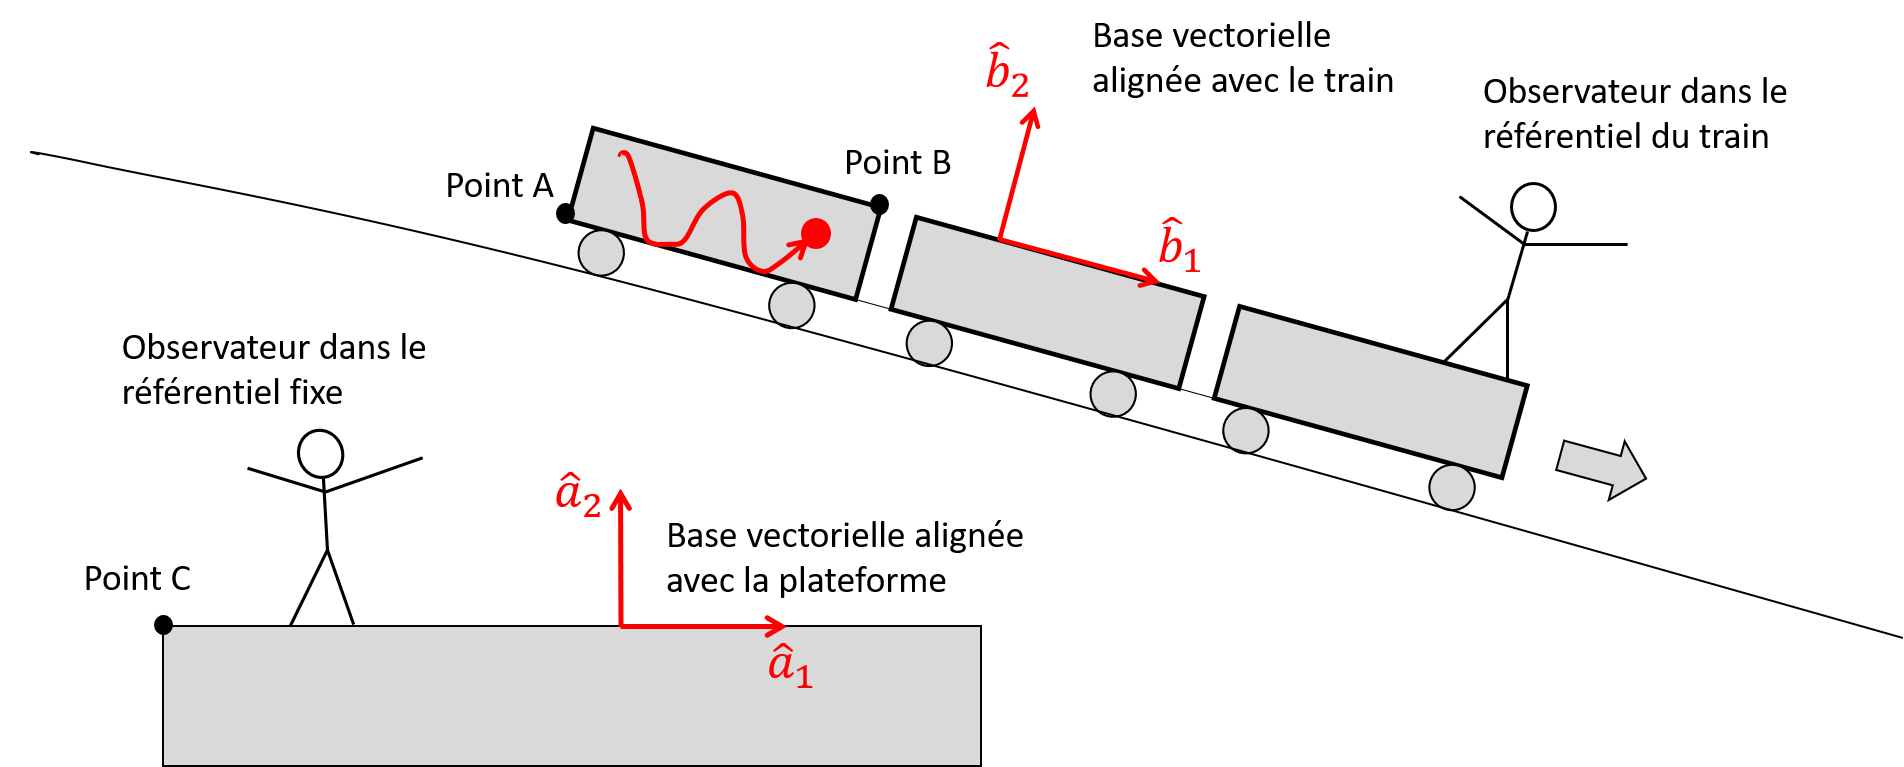
\includegraphics[width=0.90\textwidth]{train.png}
	\caption{Exemple de référentiels, points d'origine et bases vectorielles}
	\label{fig:train}
\end{figure}
%%%%%%%%%%%%%%%%%%%%%%%%%%%%%%%%%%%%%%%%%%%%%%%%%%%%%%%%%%%%%%%%%%%%%%%%%%%%%%%

La figure \ref{fig:train} illustre ces concepts par un exemple où un train descend une pente à vitesse constante et un ballon rebondit sur le sol du troisième wagon. Deux bases vectorielles sont définies, une alignée avec l'horizontale et une alignée avec le train. Plusieurs points d'origine pour les mesures de position sont aussi disponibles. Finalement, deux référentiels sont définis, un référentiel attaché à la Terre (fixe) et un référentiel qui est attaché au train. Les coordonnées d'un vecteur-colonne qui décris la position du ballon:
%%%%%%%%%%%%%%%%%%%%%%%%%%%%%%%%%%%%%
\begin{equation}
\col{r}_{Ball} = \left[ \begin{array}{c} r_1 \\ r_2 \end{array} \right]
\end{equation}
%%%%%%%%%%%%%%%%%%%%%%%%%%%%%%%%%%%%%
sont illustrés pour différents choix d'origine et de base vectorielle, lorsque que le référentiel fixe est utilisé (figure \ref{fig:refex1}) et lorsque que le référentiel du train est utilisé (figure \ref{fig:refex2}). Il est à noter que les points d'origine sont ici fixés à la Terre lorsque le référentiel fixe est utilisé, et fixés au train lorsque que le référentiel du train est utilisé. Comme illustré pour cet exemple, \textbf{un changement d'origine est analogue à une translation} de la trajectoire, \textbf{un changement de base vectorielle est analogue à une rotation} de la trajectoire, et \textbf{un changement de référentiel est ici analogue à une dilatation} de la trajectoire dans la direction $\hat{b}_1$, qui correspond à la direction de la vitesse du train. 

%%%%%%%%%%%%%%%%%%%%%%%%%%%%%%%%%%%%%%%%%%%%%%%%%%%%%%%%%%%%%%%
\begin{figure}[H]
				%\vspace{-10pt}
        \centering
        \subfloat[Repère $\{ A, \hat{a}_1, \hat{a}_2, \hat{a}_3\}$]{
				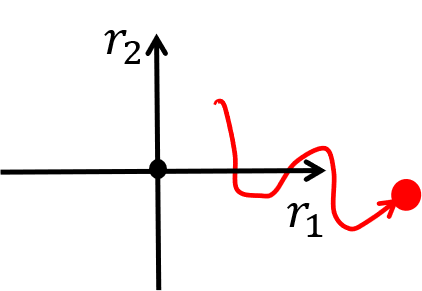
\includegraphics[width=0.23\textwidth]{ref_fixe_r_a_A.png}
				} \hspace{20pt}
				\subfloat[Repère $\{ B, \hat{a}_1, \hat{a}_2, \hat{a}_3\}$]{
				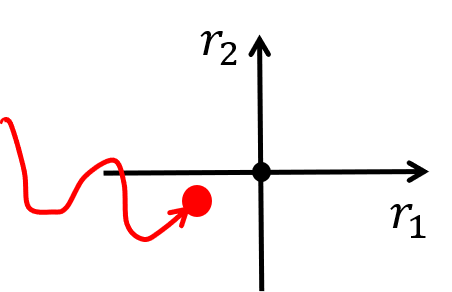
\includegraphics[width=0.24\textwidth]{ref_fixe_r_a_B.png}
				} \hspace{190pt}
				\subfloat[Repère $\{ A, \hat{b}_1, \hat{b}_2, \hat{b}_3\}$]{
				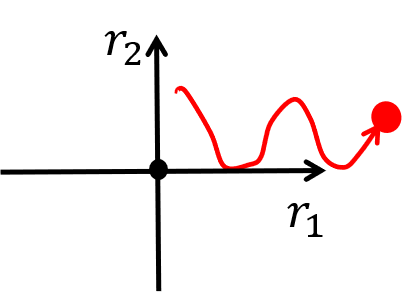
\includegraphics[width=0.22\textwidth]{ref_fixe_r_b_A.png}
				} \hspace{20pt}
				\subfloat[Repère $\{ B, \hat{b}_1, \hat{b}_2, \hat{b}_3\}$]{
				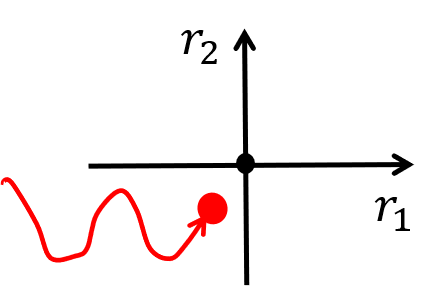
\includegraphics[width=0.24\textwidth]{ref_fixe_r_b_B.png}
				}
        \caption{Trajectoire du ballon avec un repère attaché au \textbf{référentiel fixe}}
				\label{fig:refex1}
\end{figure}
%%%%%%%%%%%%%%%%%%%%%%%%%%%%%%%%%%%%%%%%%%%%%%%%%%%%%%%%%%%%%%%%%

%%%%%%%%%%%%%%%%%%%%%%%%%%%%%%%%%%%%%%%%%%%%%%%%%%%%%%%%%%%%%%%
\begin{figure}[H]
				%\vspace{-10pt}
        \centering
				\subfloat[Repère $\{ A, \hat{a}_1, \hat{a}_2, \hat{a}_3\}$]{
				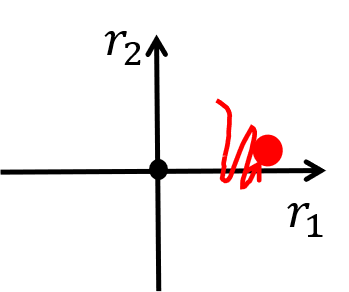
\includegraphics[width=0.22\textwidth]{ref_train_r_a_A.png}
				} \hspace{20pt}
				\subfloat[Repère $\{ B, \hat{a}_1, \hat{a}_2, \hat{a}_3\}$]{
				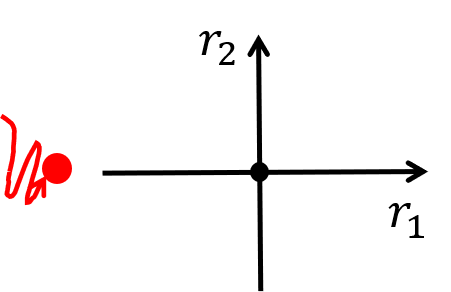
\includegraphics[width=0.25\textwidth]{ref_train_r_a_B.png}
				} \hspace{190pt}
				\subfloat[Repère $\{ A, \hat{b}_1, \hat{b}_2, \hat{b}_3\}$]{
				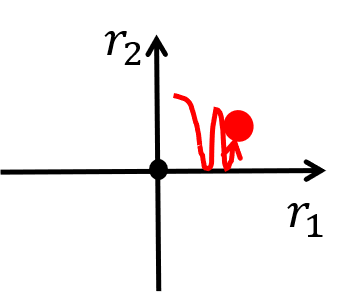
\includegraphics[width=0.22\textwidth]{ref_train_r_b_A.png}
				} \hspace{20pt}
				\subfloat[Repère $\{ B, \hat{b}_1, \hat{b}_2, \hat{b}_3\}$]{
				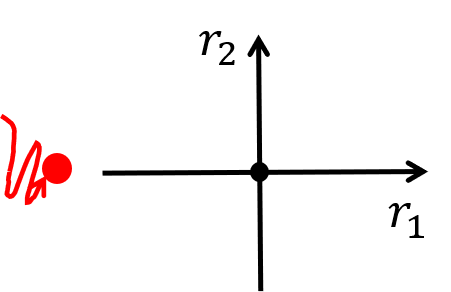
\includegraphics[width=0.25\textwidth]{ref_train_r_a_B.png}
				}
        \caption{Trajectoire du ballon avec un repère attaché au \textbf{référentiel du train}}
				\label{fig:refex2}
\end{figure}
%%%%%%%%%%%%%%%%%%%%%%%%%%%%%%%%%%%%%%%%%%%%%%%%%%%%%%%%%%%%%%%%%



%%%%%%%%%%%%%%%%%%%%%%%%%%%%%%%%%%%%%%%%%%%%%%%%%%%%%%%%%%%%%%
\newpage
\section{Vitesse et dérivée d'un vecteur position} 
%%%%%%%%%%%%%%%%%%%%%%%%%%%%%%%%%%%%%%%%%%%%%%%%%%%%%%%%%%%%%%

À venir!

Notes: 

comparaison entre l'approche vectorielle et l'approche avec les composantes


%%%%%%%%%%%%%%%%%%%%%%%%%%%%%%%%%%%%%%%%%%%%%%%%%%%%%%%%%%%%%%%%%%%%%%%%%%%%%%%%%%%%%%%%%%%%%%%%%%%%%%%%%%%%%%%%
\newpage
\section{Vitesse angulaire et dérivée d'une matrice de rotation}
%%%%%%%%%%%%%%%%%%%%%%%%%%%%%%%%%%%%%%%%%%%%%%%%%%%%%%%%%%%%%%%%%%%%%%%%%%%%%%%%%%%%%%%%%%%%%%%%%%%%%%%%%%%%%%%%

%%%%%%%%%%%%%%%%
\begin{equation}
\dot{R} = \frac{d}{dt} R = \col{w}^x \, R
\end{equation}
%%%%%%%%%%%%%%%

À venir!

%%%%%%%%%%%%%%%%%%%%%%%%%%%%%%%%%%%%%%%%%%%%%%%%%%%%%%%%%%%%%%%%%%%%%%%%%%%%%%%%%%%%%%%%%%%%%%%%%
\newpage
\section{Cinématique différentielle des robots manipulateurs}
\label{sec:differentialkinematicmanipulators}
%%%%%%%%%%%%%%%%%%%%%%%%%%%%%%%%%%%%%%%%%%%%%%%%%%%%%%%%%%%%%%%%%%%%%%%%%%%%%%%%%%%%%%%%%%%%%%%%%


La cinématique différentielle c'est l'étude de la relation entre le mouvement des joints et le mouvement associé de l'effecteur. Dans le chapitre \ref{sec:cine1}, les fonctions reliant la position de l'effecteur $\col{r}$ et la configuration du robot dans l'espace des joints $\col{q}$ ont été étudiées:
%%%%%%%%%%%%%%%%
\begin{equation}
\text{Cinématique directe:}  \quad \col{r} = f\left( \, \col{q} \, \right)  \quad  \text{inverse:} \quad \col{q} = f^{-1}\left( \, \col{r}  \, \right) 
\end{equation}
%%%%%%%%%%%%%%%

Plusieurs méthodes en robotique sont plutôt basées sur les fonctions qui relient la vitesse de l'effecteur $\col{\dot{r}}$ à la vitesse des joints $\col{\dot{q}}$. Ces fonctions prennent la forme suivante:
%%%%%%%%%%%%%%%%
\begin{equation}
\text{Cinématique différentielle directe:} \quad \col{\dot{r}} = J\left( \, \col{q} \, \right) \, \col{\dot{q}}   \quad \text{inverse:} \quad \col{\dot{q}} = J^{-1}\left( \, \col{q} \, \right) \, \col{\dot{r}}
\end{equation}
%%%%%%%%%%%%%%%
Les fonctions de cinématique différentielle impliquent une matrice Jacobienne qui relit des déplacements infinitésimales des joints aux déplacements infinitésimales de l'effecteur:
%%%%%%%%%%%%%%%%
\begin{equation}
\text{Matrice Jacobienne:} \quad J\left( \col{q} \right) = \frac{\partial \col{r}}{\partial \col{q}} = 
\left[ \begin{array}{c c c} 
\frac{\partial r_1 }{\partial q_1}   &  \hdots & \frac{\partial r_1 }{\partial q_n} \\ 
\vdots                               &  \ddots & \vdots                             \\
\frac{\partial r_m }{\partial q_1}   &  \hdots & \frac{\partial r_m }{\partial q_n}
\end{array} \right]_{m \times n}
\end{equation}
%%%%%%%%%%%%%%%%
ou $n$ est le nombre de joints, i.e. le nombre de DDL du robot, et $m$ est le nombre de coordonnées de l'espace sortie, par exemple la pose de l'effecteur.  D'un point de vue mathématique, la matrice Jacobienne $J$ correspond au gradient de la fonction multi-variable $\col{r} = f\left( \, \col{q} \, \right)$. Plus de détails sur la dérivation dans un contexte multi-variable sont disponibles à la section \ref{sec:vecmatdifferentiation}.

La composante $J_{ij}$ de la matrice correspond à la variation de la coordonnée $r_i$ de l'effecteur, due à un déplacement unitaire du joint $q_j$. La relation entre les déplacements infinitésimales est données par:
%%%%%%%%%%%%%%%%%%%%
\begin{align}
%%%%%%%%%%%%%%%%%%%%
%d\col{r}  = J(\col{q}) d\col{q}
\left[ \begin{array}{c}  \\ d\col{r} \\ \\
\end{array} \right]_{m \times 1}
&= 
\left[ \begin{array}{c c c} 
&&\\
& J(\col{q}) &\\
&&
\end{array} \right]_{m \times n}
\left[ \begin{array}{c} 
\\ d\col{q} \\ \\
\end{array} \right]_{n \times 1}
%%%%%%%%%%%%%%%%%%%%
\quad \Leftrightarrow \quad
%%%%%%%%%%%%%%%%%%%%
%\underbrace{
dr_j
%}_{mouvement de l'effecteur selon l'axe $j$}
%\underbrace{
= \sum_i^n{
%}_{somme des contributions des joints}
%\underbrace{
J_{ji} 
%}_{bras de levier}
%\underbrace{
dq_i
%}_{mouvement du joint $i$}
}
\quad \quad j \in \left\{ 1 , ... , m \right\}
\label{eq:diffkin1}
%%%%%%%%%%%%%%%%%%%%
\end{align}
%%%%%%%%%%%%%%%%%%%%


La relation qui relit les vitesses est relié à la relation entre les déplacements infinitésimales par le principe des dérivées en chaînes:
%%%%%%%%%%%%%%%%
\begin{equation}
\text{Dérivées en chaînes:} 
\underbrace{
\frac{d \col{r}}{dt}
}_{\col{\dot{r}}}
= 
\underbrace{
\left( \frac{\partial \col{r}}{\partial \col{q}} \right)
}_{J(\col{q})}
\underbrace{
\frac{d \col{q}}{dt}
}_{\col{\dot{q}}}
\end{equation}
%%%%%%%%%%%%%%%%
autrement dit, il suffit de diviser l'équation \eqref{eq:diffkin1} par $dt$ pour obtenir la relation entres les vitesses. 

%%%%%%%%%%%%%%%%%%%%%%%%%%%%%%%%%%%%%%%%%%%%%%%%%%%%%%%%%%%%%%%%%%%%%%%%%%%%%%%%%%%%%%%%%%%%%%%%%
\subsection{La matrice Jacobienne}
%%%%%%%%%%%%%%%%%%%%%%%%%%%%%%%%%%%%%%%%%%%%%%%%%%%%%%%%%%%%%%%%%%%%%%%%%%%%%%%%%%%%%%%%%%%%%%%%%

\paragraph{Unités} Typiquement pour les analyse de cinématique différentielle, les variables de sortie sont les DDL de translation de l'effecteur, la pose complète de l'effecteur ou bien des variables qui décrivent les DDL de l'espace de la tâche; et les variables d'entrée sont les vitesse angulaire des joints du robot. Les unités des composantes $J_{ij}$ de la matrice Jacobienne associée sont donc typiquement soit des unités de distance qui correspondent à des \textit{bras de levier}, ou bien des ratios adimensionnels de vitesses angulaires. 

\paragraph{Non-linéarité} Il est important de noter que généralement la matrice Jacobienne est une fonction de la configuration $\col{q}$ du robot. Comme la fonction de cinématique directe est généralement hautement non-linéaire, l'effet d'un déplacement infinitésimal d'un joint sur l'effecteur dépend considérablement de la configuration initiale. La matrice Jacobienne est donc seulement valide pour décrire des petites variation déplacement autour de la configuration pour laquelle elle a été évaluée, ou bien pour la relation entre les vitesses momentanément à cette configuration. 

\paragraph{Colonnes} Comme illustré à la Figure \ref{fig:jaco_graph}, dans le contexte de cinématique différentiel, la colonne $j$ de la matrice Jacobienne correspond à un vecteur déplacement de l'effecteur due au mouvement du joint $j$. 

%%%%%%%%%%%%%%%%%%%%%%%%%%%%%%%%%%%%%%%%%%%%%%%%%%
%\begin{figure}[H]
	%\centering
		%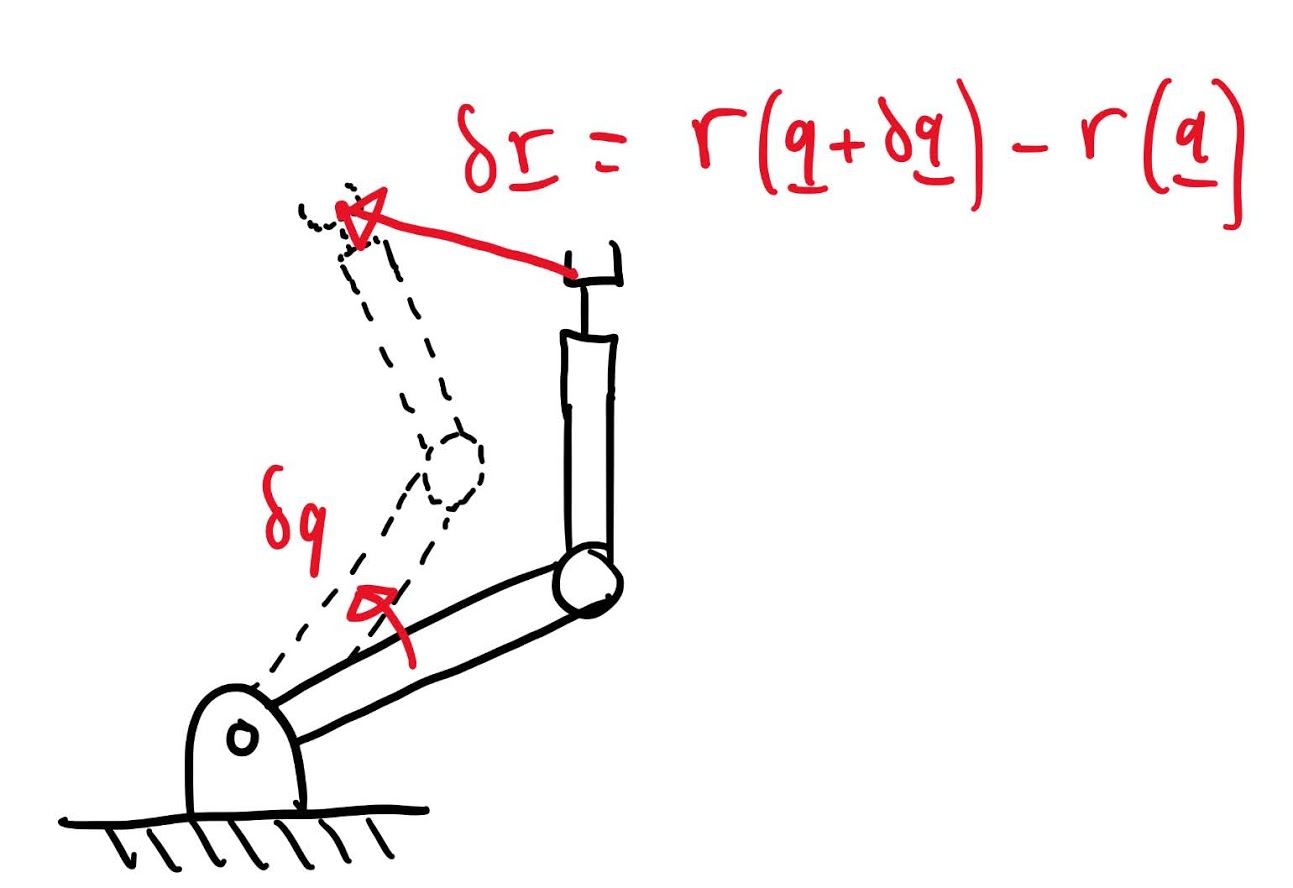
\includegraphics[width=0.75\textwidth]{diff_kin.jpg}
	%\caption{Cinématique différentielle}
	%\label{fig:diff_kin}
%\end{figure}
%%%%%%%%%%%%%%%%%%%%%%%%%%%%%%%%%%%%%%%%%%%%%%%%%%


%%%%%%%%%%%%%%%%%%%%%%%%%%%%%%%%%%%%%%%%%%%%%%%%%
\begin{figure}[H]
\vspace{-5pt}
	\centering
		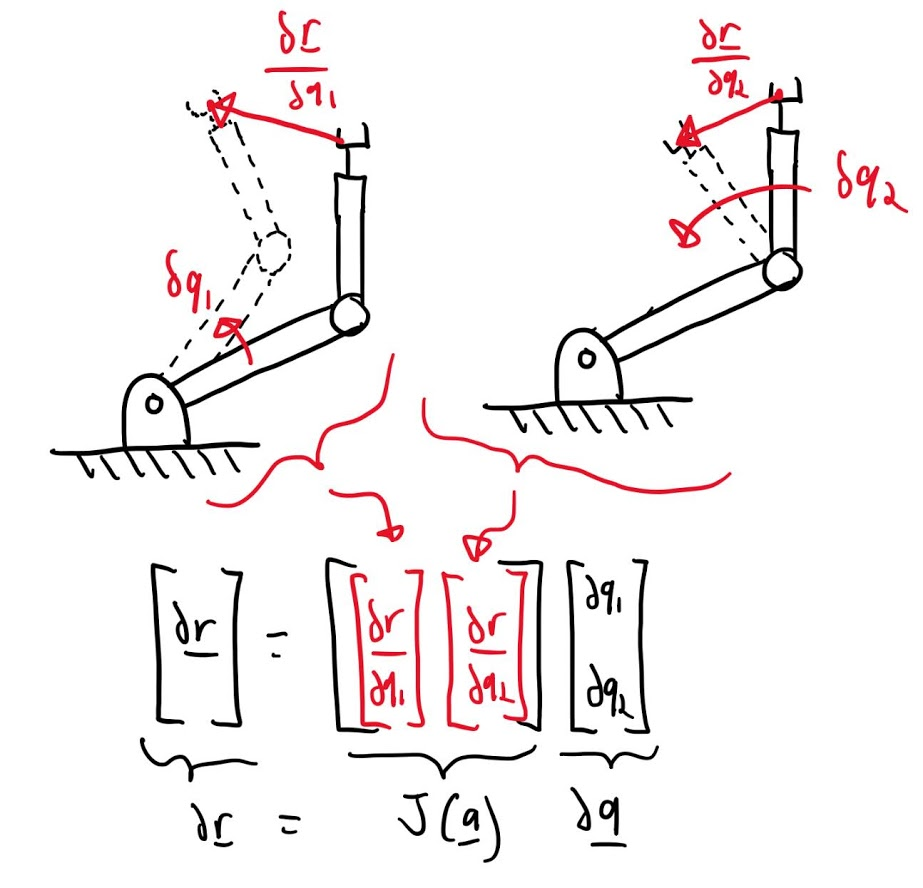
\includegraphics[width=0.55\textwidth]{jaco_graph.jpg}
	\caption{Illustration vectorielle du Jacobian du manipulateur}
	\vspace{-5pt}
	\label{fig:jaco_graph}
\end{figure}
%%%%%%%%%%%%%%%%%%%%%%%%%%%%%%%%%%%%%%%%%%%%%%%%%


%%%%%%%%%%%%%%%%%%%%%%%%%%%%%%%%%%%%%%%%%%%%%%%%%%%%%%%%%%%%%%%%%%%%%%%%%%%%%%%%%%%%%%%%%%%%
\newpage
\subsection{Cinématique différentielle incluant l'orientation de l'effecteur}
\label{sec:cindiff}
%%%%%%%%%%%%%%%%%%%%%%%%%%%%%%%%%%


%%%%%%%%%%%%%%%%%%%%%%%%%%%%%%%%%%%%%%%%%%%%%%%%%%%%%%%%%%%%%%%%%%%%%%%%%%%%%%%%%%%%%%%%%%%%%
\newpage
\subsection{Méthode de calcul du Jacobian}


\subsection{Dérivée partielle}

TODO

\subsection{Produits vectoriels}

TODO

\subsubsection{Basé sur les paramètres DH}

TODO

voir Sciciliano p.112



\newpage
%%%%%%%%%%%%%%%%%%%%%%%%%%%%%%%%%%%%%%%%%%%%%%%%%%%%%%%%%%%%%%%%%%%%%%%%%%%%%%%%%%%%%%%%%%%%%%%%%%%%%%%%%
\subsection{Exemples de cinématique différentielle pour des robots manipulateurs}

%%%%%%%%%%%%%%%%%%%%%%%%%%%%%%%%%%%%%%%%%%%%%%%%%%%%%%%%%%%%%%%%%%%%%%%%%%%%%%%%%%%%%%%%%%%%%%%%%%%%%%%%%
\subsubsection{Cinématique différentielle d'un robot cartésien}

La Figure \ref{fig:jaco_robot_cart} illustre un robot planaire constitué de deux actionneurs linéaires basé sur des vis à billes qui sont assemblés à 90 degrées. 
%%%%%%%%%%%%%%%%%%%%%%%%%%%%%%%%%%%%%%%%%%%%%%%%%
\begin{figure}[H]
	\vspace{-5pt}
	\centering
		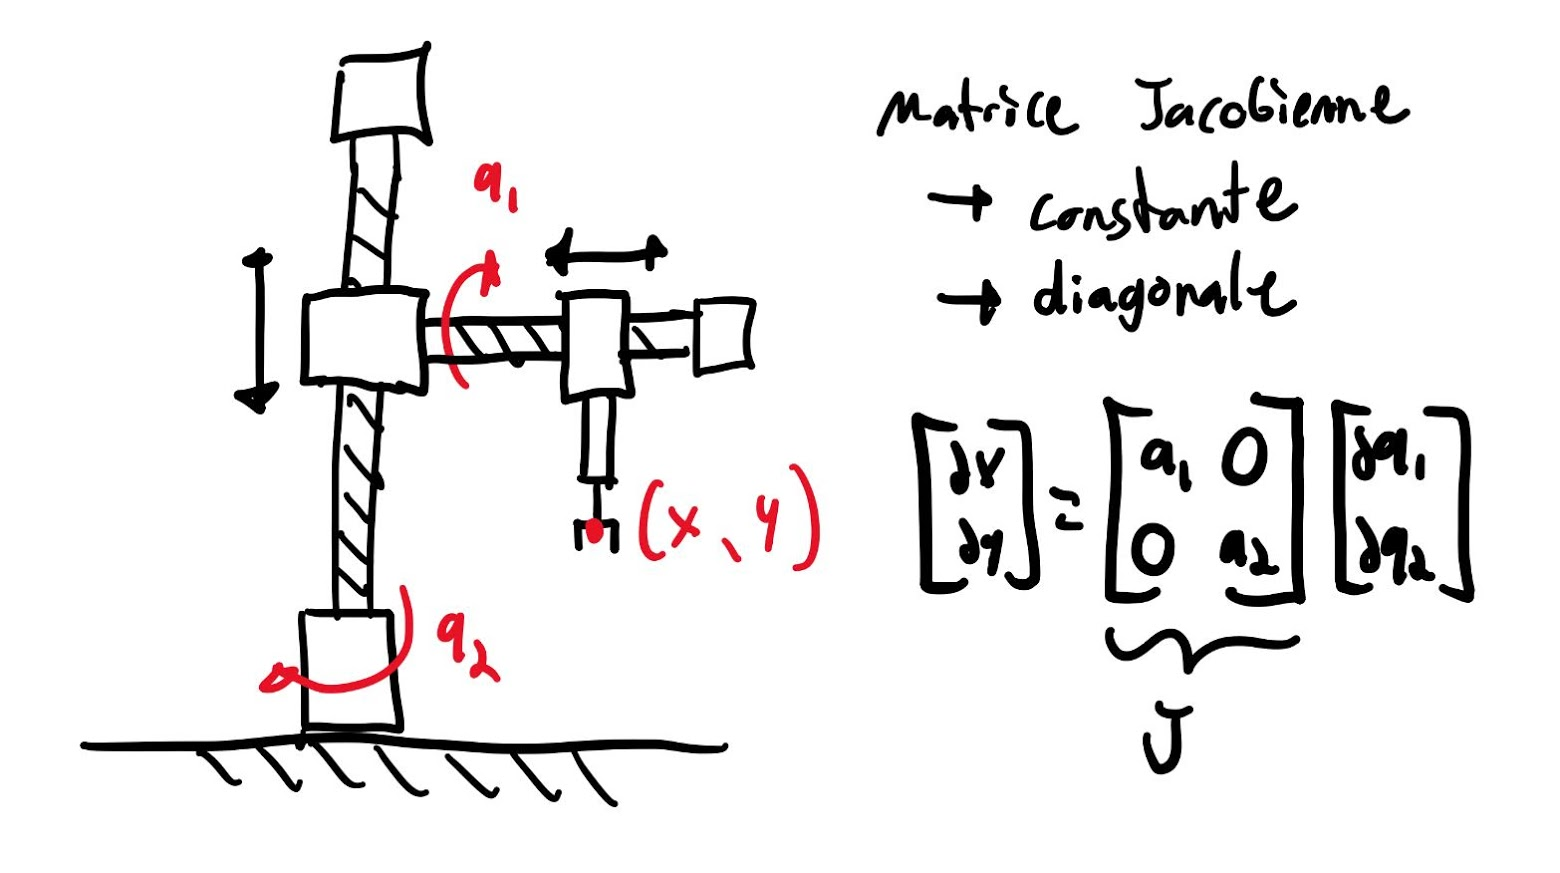
\includegraphics[width=0.65\textwidth]{jaco_robot_cart.jpg}
	\caption{Jacobien pour un robot cartésien}
	\vspace{-5pt}
	\label{fig:jaco_robot_cart}
\end{figure}
%%%%%%%%%%%%%%%%%%%%%%%%%%%%%%%%%%%%%%%%%%%%%%%%%

Pour ce robot, chaque actionneur linéaire contrôle de façon indépendante la translation $x$ et $y$ de l'effecteur, la fonction de cinématique directe est donnée par :
%%%%%%%%%%%%%%%%
\begin{align}
\quad \col{r} &= f\left( \, \col{q} \, \right)  \\
\left[ \begin{array}{c} x \\ y  \end{array} \right]  &= \left[ \begin{array}{c} a_1 q_1 \\ a_2 q_2  \end{array} \right]
\label{eq:fwdkinlin}
\end{align}
%%%%%%%%%%%%%%%
ou les variables $a_i$ sont des constantes qui relient la rotation angulaire des vis aux déplacements linéaires. La relation différentielle peut alors être calculée:
%%%%%%%%%%%%%%%%%%%%%%%%%%%%%%%%%%%
\begin{align}
\underbrace{ \left[ \begin{array}{c} \dot{x} \\ \dot{y}  \end{array} \right] }_{\dot{\col{r}}}
 &= 
\underbrace{ \left[ \begin{array}{c c } 
\frac{\partial x }{\partial q_1}   & \frac{\partial x }{\partial q_2} \\ 
\frac{\partial y }{\partial q_1}   & \frac{\partial y }{\partial q_2}
\end{array} \right]  }_{ J } 
\underbrace{ \left[ \begin{array}{c} 
\dot{q}_1 \\ 
\dot{q}_2 
\end{array} \right]}_{ \dot{\col{q}} } \\
%%%%%%%%%%%%%
\underbrace{ \left[ \begin{array}{c} \dot{x} \\ \dot{y}  \end{array} \right] }_{\dot{\col{r}}}
 &= 
\underbrace{ \left[ \begin{array}{c c } 
a_1 & 0 \\ 
0   & a_2
\end{array} \right]  }_{ J } 
\underbrace{ \left[ \begin{array}{c} 
\dot{q}_1 \\ 
\dot{q}_2 
\end{array} \right]}_{ \dot{\col{q}} } \\
\end{align} 
%%%%%%%%%%%%%%%%%%%%%%%%%%%%%%%%%%%

Il est a noter ici que: \textbf{1)} la matrice Jacobienne est diagonale car chaque joint influence indépendamment un seul DDL de l'effecteur. \textbf{2)} la matrice Jacobienne est constante et indépendante de $\col{q}$ car la relation de cinématique directe, voir équation \eqref{eq:fwdkinlin}, est linéaire. 


%%%%%%%%%%%%%%%%%%%%%%%%%%%%%%%%%%%%%%%%%%%%%%%%%%%%%%%%%%%%%%%%%%%%%%%%%%%%%%%%%%%%%%%%%%%%%%%%%%%%%%%%%
\subsubsection{Cinématique différentielle d'un robot à deux joints}
\label{sec:kindiff_2dof}

%%%%%%%%%%%%%%%%%%%%%%%%%%%%%%%%%%%%%%%%%%%%%%%%%
\begin{figure}[H]
	\centering
		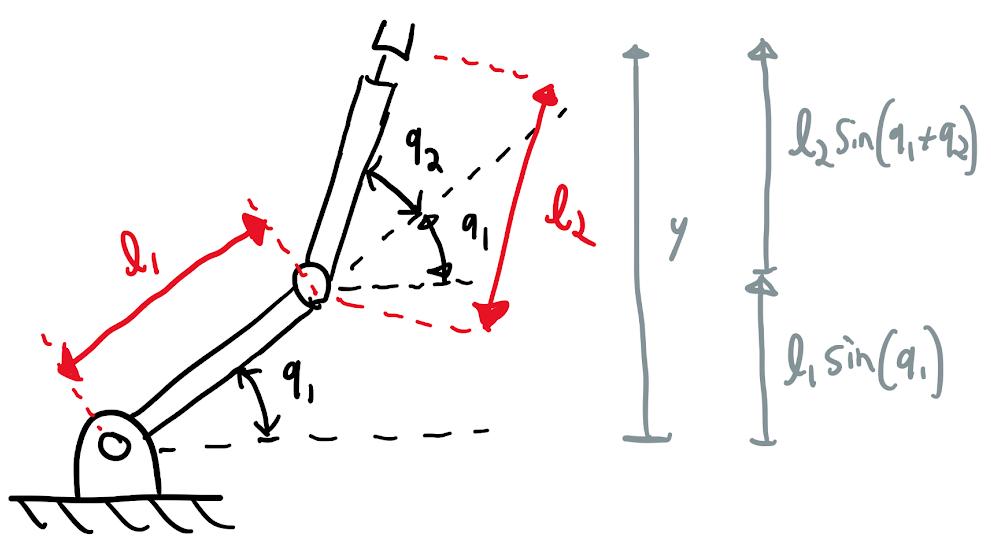
\includegraphics[width=0.65\textwidth]{robot_2dof.png}
	\caption{Robot à deux joints}
	\label{fig:robot_2dof}
\end{figure}
%%%%%%%%%%%%%%%%%%%%%%%%%%%%%%%%%%%%%%%%%%%%%%%%%

Pour un robot manipulateur planaire à deux DDL, comme illustré à la Figure \ref{fig:robot_2dof}, la fonction de cinématique directe est données par:
%%%%%%%%%%%%%%%%%%%%%%%%%%%%%%%%%%%
\begin{align}
\col{r} &= \left[ \begin{array}{c} x \\ y  \end{array} \right]  = \left[ \begin{array}{c} 
 l_1 c_1 + l_2 c_{12} \\ 
 l_1 s_1 + l_2 s_{12}  
\end{array} \right] 
\label{eq:kinfwd2dof}
\end{align} 
%%%%%%%%%%%%%%%%%%%%%%%%%%%%%%%%%%%
avec
%%%%%%%%%%%%%%%%%%%%%%%%%%%%%%%%%%%
\begin{align}
c_1    &= \cos( q_1 ) \\
s_1    &= \sin( q_1 ) \\
c_{12} &= \cos( q_1 + q_2 ) \\
s_{12} &= \sin( q_1 + q_2 )
\end{align} 
%%%%%%%%%%%%%%%%%%%%%%%%%%%%%%%%%%%

On peut alors trouver la relation différentielle en dérivant par rapport au temps:
%%%%%%%%%%%%%%%%%%%%%%%%%%%%%%%%%%%
\begin{align}
\dot{\col{r}} &= \frac{d\col{r}}{dt} = \left[ \begin{array}{c} \dot{x} \\ \dot{y}  \end{array} \right]  = \left[ \begin{array}{c} 
-l_1 s_1 \dot{q}_1 - l_2 s_{12}( \dot{q}_1 + \dot{q}_2 ) \\ 
 l_1 c_1 \dot{q}_1 + l_2 c_{12}( \dot{q}_1 + \dot{q}_2 )  
\end{array} \right] \\
\dot{\col{r}}  &= 
\underbrace{ \left[ \begin{array}{c c } 
-l_1 s_1 - l_2 s_{12} & - l_2 s_{12} \\ 
 l_1 c_1 + l_2 c_{12} &   l_2 c_{12}
\end{array} \right]  }_{ J(\col{q}) } 
\underbrace{ \left[ \begin{array}{c} 
\dot{q}_1 \\ 
\dot{q}_2 
\end{array} \right]}_{ \dot{\col{q}} } \\
\dot{\col{r}}  &= J(\col{q}) \dot{\col{q}}
\end{align} 
%%%%%%%%%%%%%%%%%%%%%%%%%%%%%%%%%%%



\newpage
%%%%%%%%%%%%%%%%%%%%%%%%%%%%%%%%%%%%%%%%%%%%%%%%%%%%%%%%%%%%%%%%%%%%%%%%%%%%%%%%%%%%%%%%%%%%%%%%%%%%%%%%%
\subsubsection{Cinématique différentielle d'un robot à trois joints}
\label{sec:diffkinrobot3dofex}

Les Figures \pageref{fig:jaco_3dof_a} et \ref{fig:jaco_3dof_b} illustre la cinématique différentielle d'un robot à trois joints dans une configuration qui permet de bien visualiser indépendamment les effets du mouvement de chaque joint. 

%%%%%%%%%%%%%%%%%%%%%%%%%%%%%%%%%%%%%%%%%%%%%%%%%
\begin{figure}[H]
	\centering
		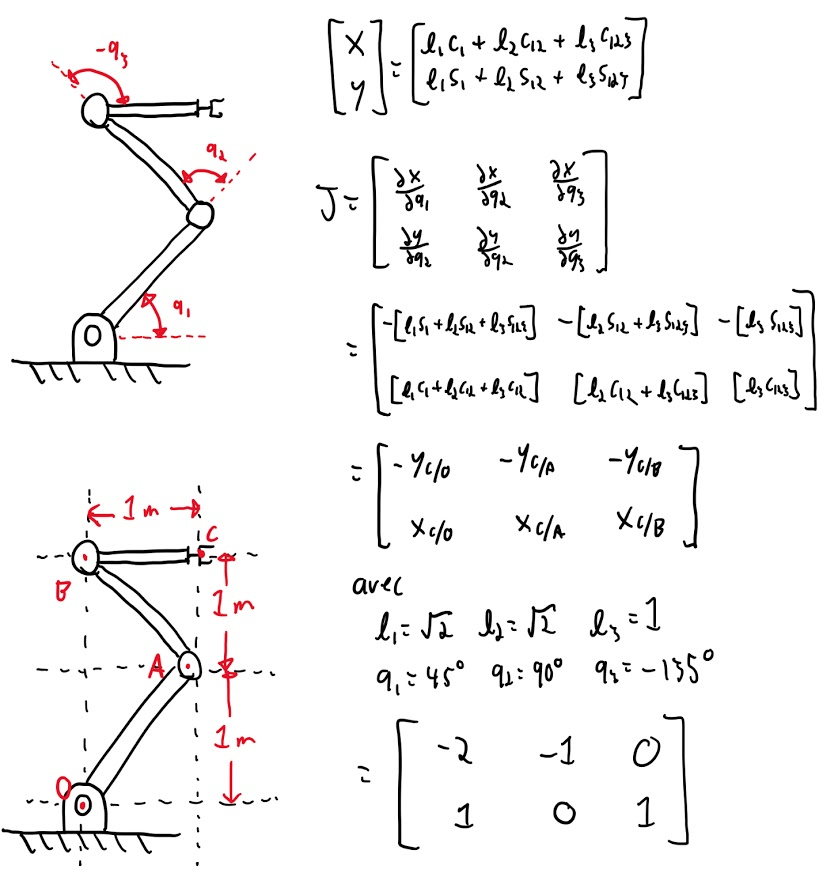
\includegraphics[width=0.75\textwidth]{jaco_3dof_a.jpg}
	\caption{Jacobien d'un robot à trois joints - partie a)}
	\label{fig:jaco_3dof_a}
\end{figure}
%%%%%%%%%%%%%%%%%%%%%%%%%%%%%%%%%%%%%%%%%%%%%%%%%

%%%%%%%%%%%%%%%%%%%%%%%%%%%%%%%%%%%%%%%%%%%%%%%%%
\begin{figure}[H]
	\centering
		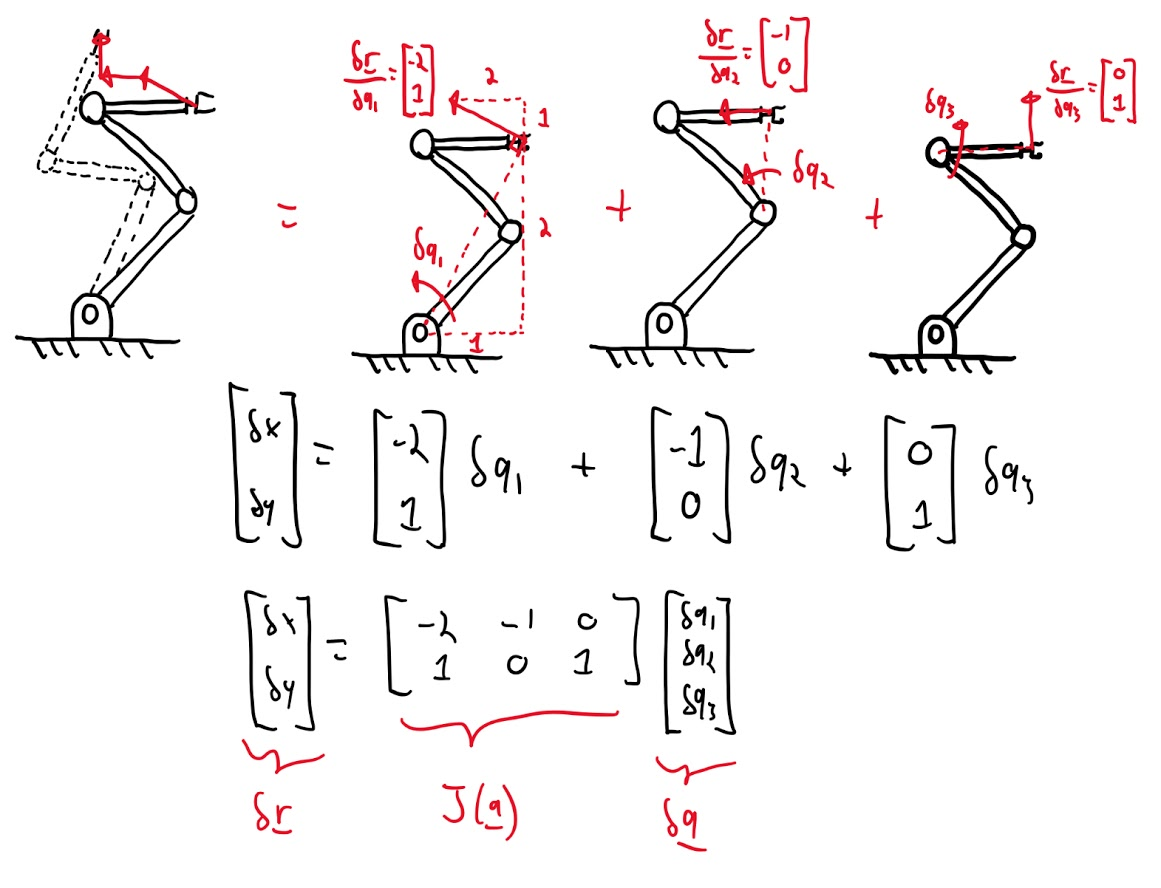
\includegraphics[width=0.85\textwidth]{jaco_3dof_b.jpg}
	\caption{Jacobien d'un robot à trois joints - partie b)}
	\label{fig:jaco_3dof_b}
\end{figure}
%%%%%%%%%%%%%%%%%%%%%%%%%%%%%%%%%%%%%%%%%%%%%%%%%



%%%%%%%%%%%%%%%%%%%%%%%%%%%%%%%%%%%%%%%%%%%%%%%%%%%%%%%%%%%%%%%%%%%%%%%%%%%%%%%%%%%%%%%%%%%%%%%%%%%%%%%%%
\subsection{Cinématique différentielle inverse}

Lorsque le problème de cinématique différentielle est inversé, c'est-à-dire lorsqu'on cherche un vecteur de vitesse aux joints $\col{\dot{q}}$ qui va produire une vitesse de l'effecteur spécifiée $\col{\dot{r}}$, il faut inverser la relation mathématique. Lorsque la matrice Jacobienne est carré et non-singulière, il suffit de multiplier la relation $\col{\dot{r}} = J\left( \, \col{q} \, \right) \, \col{\dot{q}}$ par l'inverse du Jacobien des deux côtés de l'équation pour obtenir la relation:
%
%%%%%%%%%%%%%%%%%%%%%%%%%%%%%%%%%%%
\begin{align}
\col{\dot{q}} = J^{-1}\left( \, \col{q} \, \right) \, \col{\dot{r}}
\end{align} 
%%%%%%%%%%%%%%%%%%%%%%%%%%%%%%%%%%%
%
Toutefois, cette opération est impossible si le robot a une configuration singulière (voir section \ref{sec:singu}). De plus, si les dimensions de $\col{q}$ et $\col{r}$ sont différentes, la matrice Jacobienne est rectangulaire et d'autres techniques doivent être utilisée (voir sections \ref{sec:redondant} et \ref{sec:overconstraintrobot})


%%%%%%%%%%%%%%%%%%%%%%%%%%%%%%%%%%%%%%%%%%%%%%%%%%%%%%%%%%%%%%%%%%%%%%%%%%%%%%%%%%%%%%%%%%%%%%%%%%%%%%%%%
\subsection{Les singularités}
\label{sec:singu}
%%%%%%%%%%%%%%%%%%%%%%%%%%%%%%%%%%
Certaine configuration $\col{q}$ d'un robot manipulateur peuvent être singulière, c'est-à-dire des configuration pour lesquelles il est impossible d'inverser la matrice Jacobienne. Les configurations singulière sont l'ensemble des configurations pour lesquelles le déterminant de la matrice Jacobienne est nul:
%%%%%%%%%%%%%%%%%%%%%%%%%%%%%%%%%%%
\begin{align}
\text{Singularités :} \quad \{  \col{q} \; | \; det(J(\col{q})) = 0 \}
\end{align} 
%%%%%%%%%%%%%%%%%%%%%%%%%%%%%%%%%%%
Ces situations correspondent aussi à lorsque les colonnes de $J$ sont co-linéaires, et qu'aucune combinaison linéaire ne permet de déplacer l'effecteur dans au moins une direction impossible (la matrice Jacobienne a un left-nullspace, voir section \ref{sec:leftnullspace} pour les notions d'algèbre linéaire associées). 


\subsubsection{Singularités pour un robot manipulateur 2 DDL}

Pour un robot manipulateur à deux DDl comme décrit à l'exemple \ref{sec:kindiff_2dof}, le Jacobien est donné par:
%%%%%%%%%%%%%%%%%%%%%%%%%%%%%%%%%%%
\begin{align}
J = \left[ \begin{array}{c c} 
-(l_1 s_1 + l_2 s_{12}) & - l_2 s_{12} \\
 (l_1 c_1 + l_2 c_{12}) &   l_2 c_{12}
\end{array} \right]
\end{align} 
%%%%%%%%%%%%%%%%%%%%%%%%%%%%%%%%%%%
Le déterminant de la matrice est donnée par:
%%%%%%%%%%%%%%%%%%%%%%%%%%%%%%%%%%%
\begin{align}
det(J) &= l_2 s_{12} (l_1 c_1 + l_2 c_{12}) - l_2 c_{12} (l_1 s_1 + l_2 s_{12}) \\
       &= l_1 l_2 s_{12} c_1 + l_2^2 s_{12} c_{12} - l_1 l_2 s_1 c_{12} - l_2^2 s_{12} c_{12} \\
			 &= l_1 l_2 ( s_1 c_{12} - c_1 s_{12} ) \\
			 &= l_1 l_2 s_2
\end{align} 
%%%%%%%%%%%%%%%%%%%%%%%%%%%%%%%%%%%

Donc les singularités sont les configurations avec un angle $q_2$ égale à 0 ou 180 degrés. Comme illustré à la Figure \ref{fig:sigularite_2dof}, ces configurations correspondent à lorsque les deux liens rigides du robot sont alignés. Dans ces configurations, il est seulement possible de faire bouger l'effecteur dans une direction perpendiculaire aux liens rigides. Comme illustré à la Figure \ref{fig:sigularite_2dof_b}, la direction pour laquelle le mouvement est possible correspond à l'espace colonne de la matrice Jacobienne, et la direction orthogonale pour laquelle il est impossible de déplacer l'effecteur correspond au left-nullspace de la matrice Jacobienne, voir section \ref{sec:4espfond} pour les notions d'algèbre linéaire associées.

%%%%%%%%%%%%%%%%%%%%%%%%%%%%%%%%%%
\begin{figure}[htbp]
	\centering
		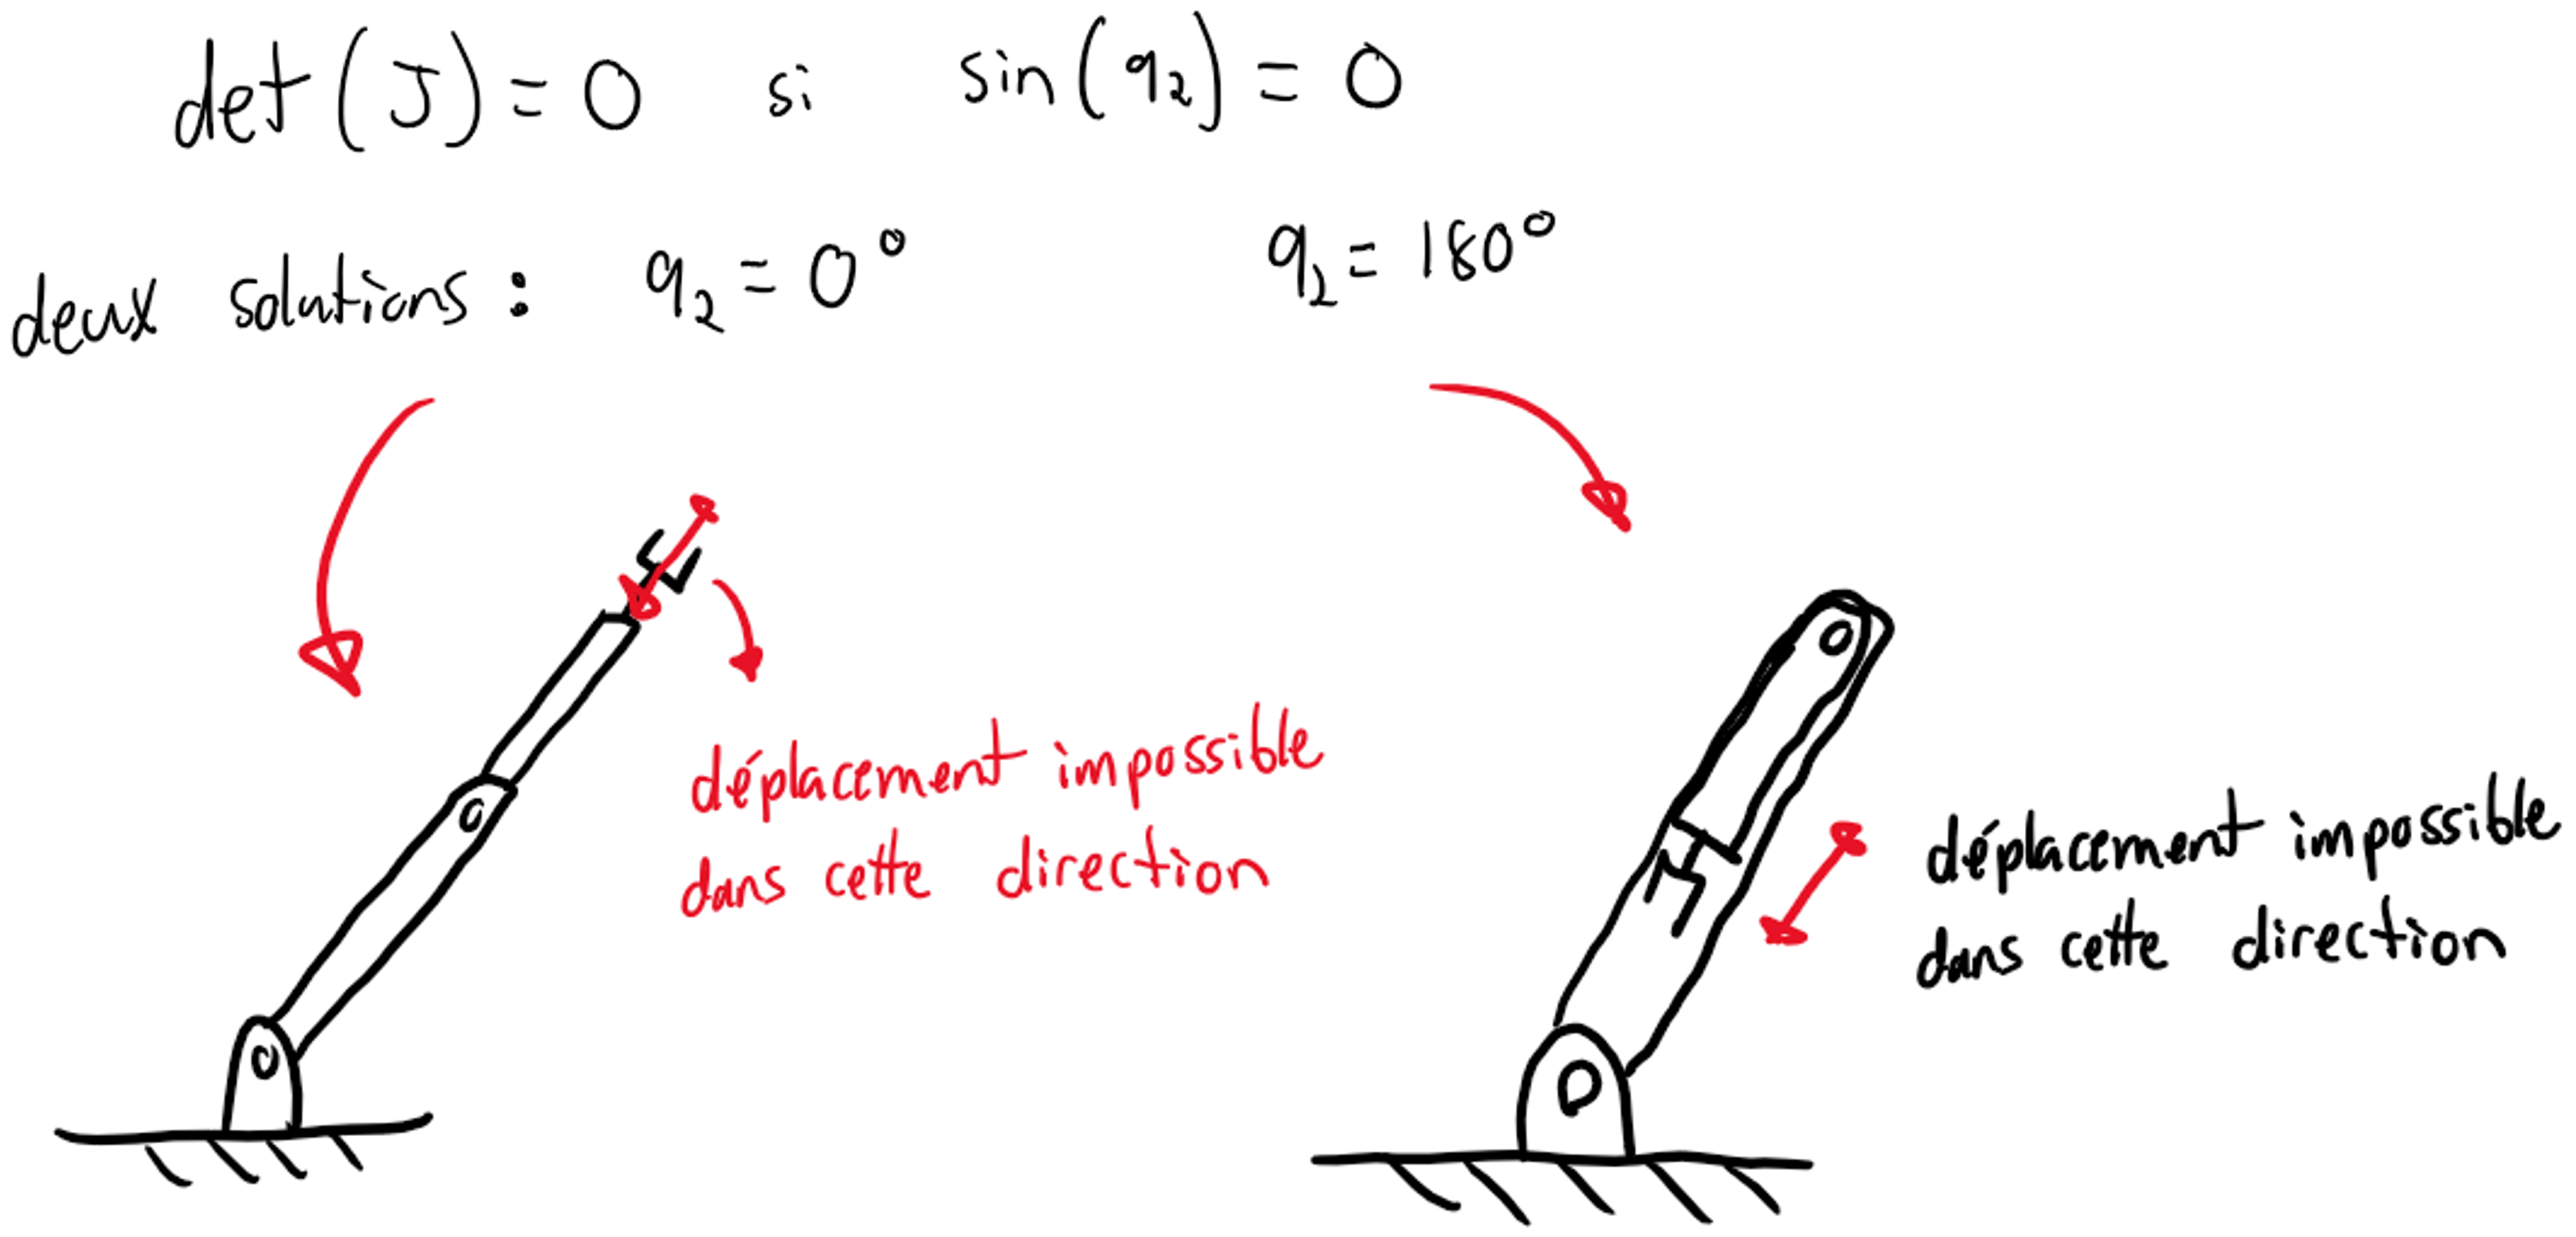
\includegraphics[width=0.75\textwidth]{sigularite_2dof.png}
	\caption{Singularités pour un robot manipulateur à deux DDL}
	\label{fig:sigularite_2dof}
\end{figure}
%%%%%%%%%%%%%%%%%%%%%%%%%%%%%%%%%%

%%%%%%%%%%%%%%%%%%%%%%%%%%%%%%%%%%
\begin{figure}[htbp]
	\centering
		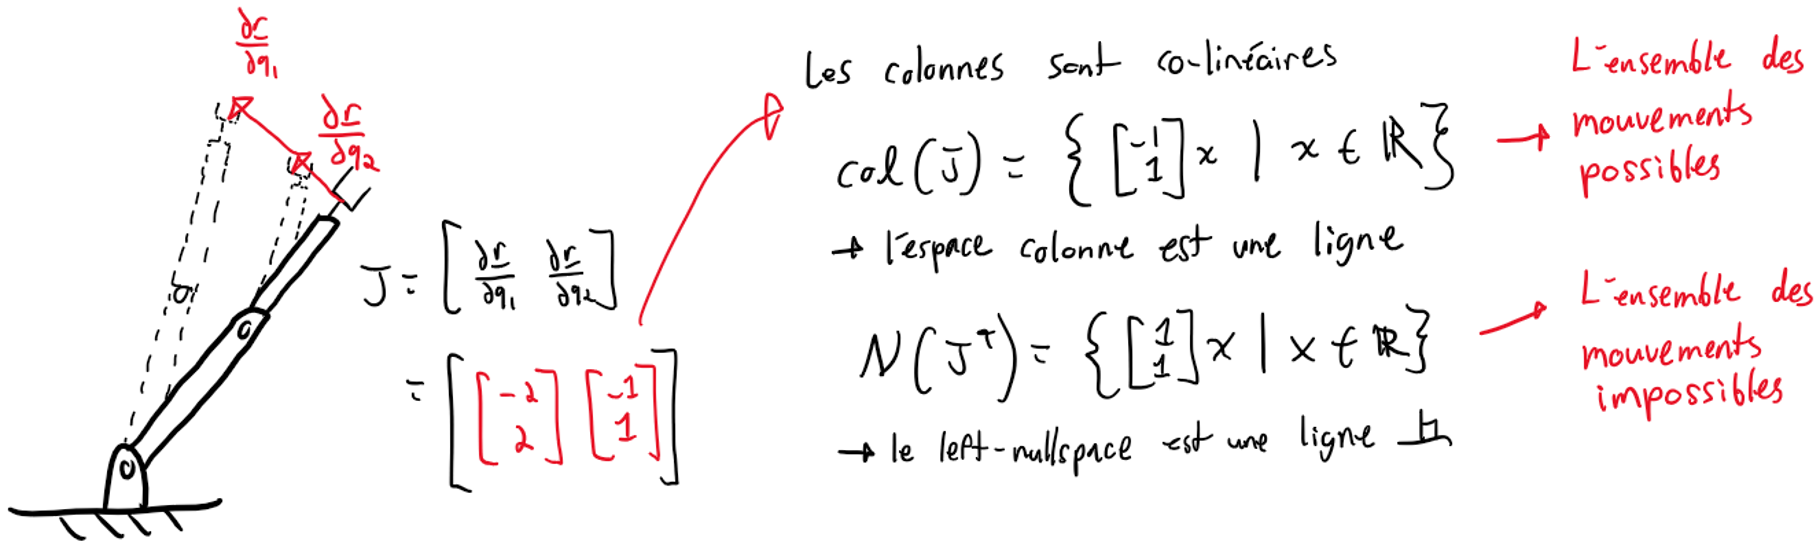
\includegraphics[width=0.95\textwidth]{sigularite_2dof_b.png}
	\caption{Co-linéarité des colonnes du Jacobien pour une singularité}
	\label{fig:sigularite_2dof_b}
\end{figure}
%%%%%%%%%%%%%%%%%%%%%%%%%%%%%%%%%%


%%%%%%%%%%%%%%%%%%%%%%%%%%%%%%%%%%%%%%%%%%%%%%%%%%%%%%%%%%%%%%%%%%%%%%%%%%%%%%%%%%%%%%%%%%%%%%%%%%%%%%%%%
\subsection{Cinématique différentielle inverse d'un robot redondant (situations sous-contraintes)}
\label{sec:invdiffkinredondant}
%%%%%%%%%%%%%%%%%%%%%%%%%%%%%%%%%%

Si le nombre d'entrées $n$ est plus grand que le nombre de sorties $m$ : 
%%%%%%%%%%%%%%%%%%%%%%%%%%%%%%%%%%%
\begin{align}
n > m
\end{align} 
%%%%%%%%%%%%%%%%%%%%%%%%%%%%%%%%%%%
avec 
%%%%%%%%%%%%%%%%%%%%%%%%%%%%%%%%%%%
\begin{align}
n &= dim(\col{q}) = \quad\text{Nombre de DDL du robot} \\
m &= dim(\col{r}) = \quad\text{Coordonnées de l'espace de la tâche} 
\end{align} 
%%%%%%%%%%%%%%%%%%%%%%%%%%%%%%%%%%%
le robot est dit redondant, et le problème de cinématique différentiel inverse est sous-contraint: il y a plusieurs solutions possible de déplacement des joints qui produisent un même déplacement de l'effecteur. Le Jacobien d'une telle situation est rectangulaire, il a plus de colonnes que de rangées:
%%%%%%%%%%%%%%%%%%%%%%%%%%%%%%%%%%%
\begin{align}
\left[ \begin{array}{c}  \\ \dot{\col{r}} \\ \\
\end{array} \right]_{m \times 1}
&= 
\left[ \begin{array}{c c c c c} 
&&&&\\
&& J(\col{q}) &&\\
&&&&
\end{array} \right]_{m \times n}
\left[ \begin{array}{c} 
\\ \\ \dot{\col{q}} \\ \\ \\
\end{array} \right]_{n \times 1}
\label{eq:underconstraintdiffkin}
\end{align} 
%%%%%%%%%%%%%%%%%%%%%%%%%%%%%%%%%%%
Cette situation nous même à un problème d'algèbre linéaire sous-contraint qui peu être résolu avec une méthode qui utilise une matrice pseudo inverse, voir section \ref{sec:pseudoinverse} pour les notions d'algèbre linéaire. Cette situation est aussi caractérisée par la présence d'un nullspace: une combinaison de déplacement des joints peut avoir un effet net nul sur l'effecteur, voir section \ref{sec:nullspace} pour les notions d'algèbre linéaire et l'exemple \ref{fig:4spaces_ex1}. 

Une méthode pour travailler avec ce genre de situation consiste à utiliser l'équation de cinématique inverse suivante:
%%%%%%%%%%%%%%%%%%%%%%%%%%%%%%%%%%%
\begin{align}
\left[ \begin{array}{c}  \\ \\ \dot{\col{q}} \\ \\ \\
\end{array} \right]_{n \times 1}
&= 
\underbrace{
\left[ \begin{array}{c c c} 
&&\\ &&\\ & J^{\#} & \\&& \\ &&
\end{array} \right]_{n \times m}
}_{\text{Pseudo-inverse}}
\left[ \begin{array}{c} 
\\ \dot{\col{r}} \\ \\
\end{array} \right]_{m \times 1} + 
\underbrace{
\left[ \begin{array}{c c c c c} 
&&&&\\ &&&&\\ && I - J^{\#}J && \\&&&& \\ &&&&
\end{array} \right]_{n \times n}
}_{\text{Projection sur le Nullspace}}
\left[ \begin{array}{c} 
\\ \\ \col{\psi} \\ \\ \\
\end{array} \right]_{n \times 1}
\label{eq:pseudoinversediffkin}
\end{align} 
%%%%%%%%%%%%%%%%%%%%%%%%%%%%%%%%%%%
avec $J^{\#}$ qui est la matrice pseudo-inverse droite de Moore–Penrose, définie par:
%%%%%%%%%%%%%%%%%%%%%%%%%%%%%%%%%%%
\begin{align}
J^{\#} = J^T\, (JJ^T)^{-1}
\end{align} 
%%%%%%%%%%%%%%%%%%%%%%%%%%%%%%%%%%%
Le premier terme $J^{\#} \col{\dot{r}}$ produit un vecteur $\col{\dot{q}}$ qui produit une solution exacte pour le système d'équations \eqref{eq:underconstraintdiffkin}
et minimise la norme du vecteur-colonne $\col{\dot{q}}$. Le second terme produit une variation pour le vecteur $\col{\dot{q}}$ qui réside dans le nullspace de la matrice $J$, donc cette variation n'a aucun influence sur la sortie et n’affectera pas l'objectif principal d'obtenir un vecteur $\col{\dot{q}}$ qui produit un mouvement de l'effecteur donné par $\col{\dot{r}}$. Le vecteur $\col{\psi}$ dans le second terme est arbitraire et peut être utilisé pour prioriser certaine solutions sans influencer la justesse de la solution. 


\newpage
%%%%%%%%%%%%%%%%%%%%%%%%%%%%%%%%%%%%%%%%%%%%%%%%%%%%%%%%%%%%%%%%%%%%%%%%%%%%%%%%%%%%%%%%%%%%%%%%%%%%%%%%%
\subsubsection{Exemple de cinématique différentielle inverse pour une situation sous-contrainte}


Le robot de l'exemple \ref{sec:diffkinrobot3dofex} est ici analysé en termes de cinématique différentielle, la Figure \ref{fig:robot_redo_a} illustre la présence de plusieurs solutions possibles et la Figure \ref{fig:robot_redo_c} illustre l'utilisation de la matrice pseudo-inverse pour obtenir la solution optimale ainsi que le nullspace. 

%%%%%%%%%%%%%%%%%%%%%%%%%%%%%%%%%%
\begin{figure}[H]
	\centering
		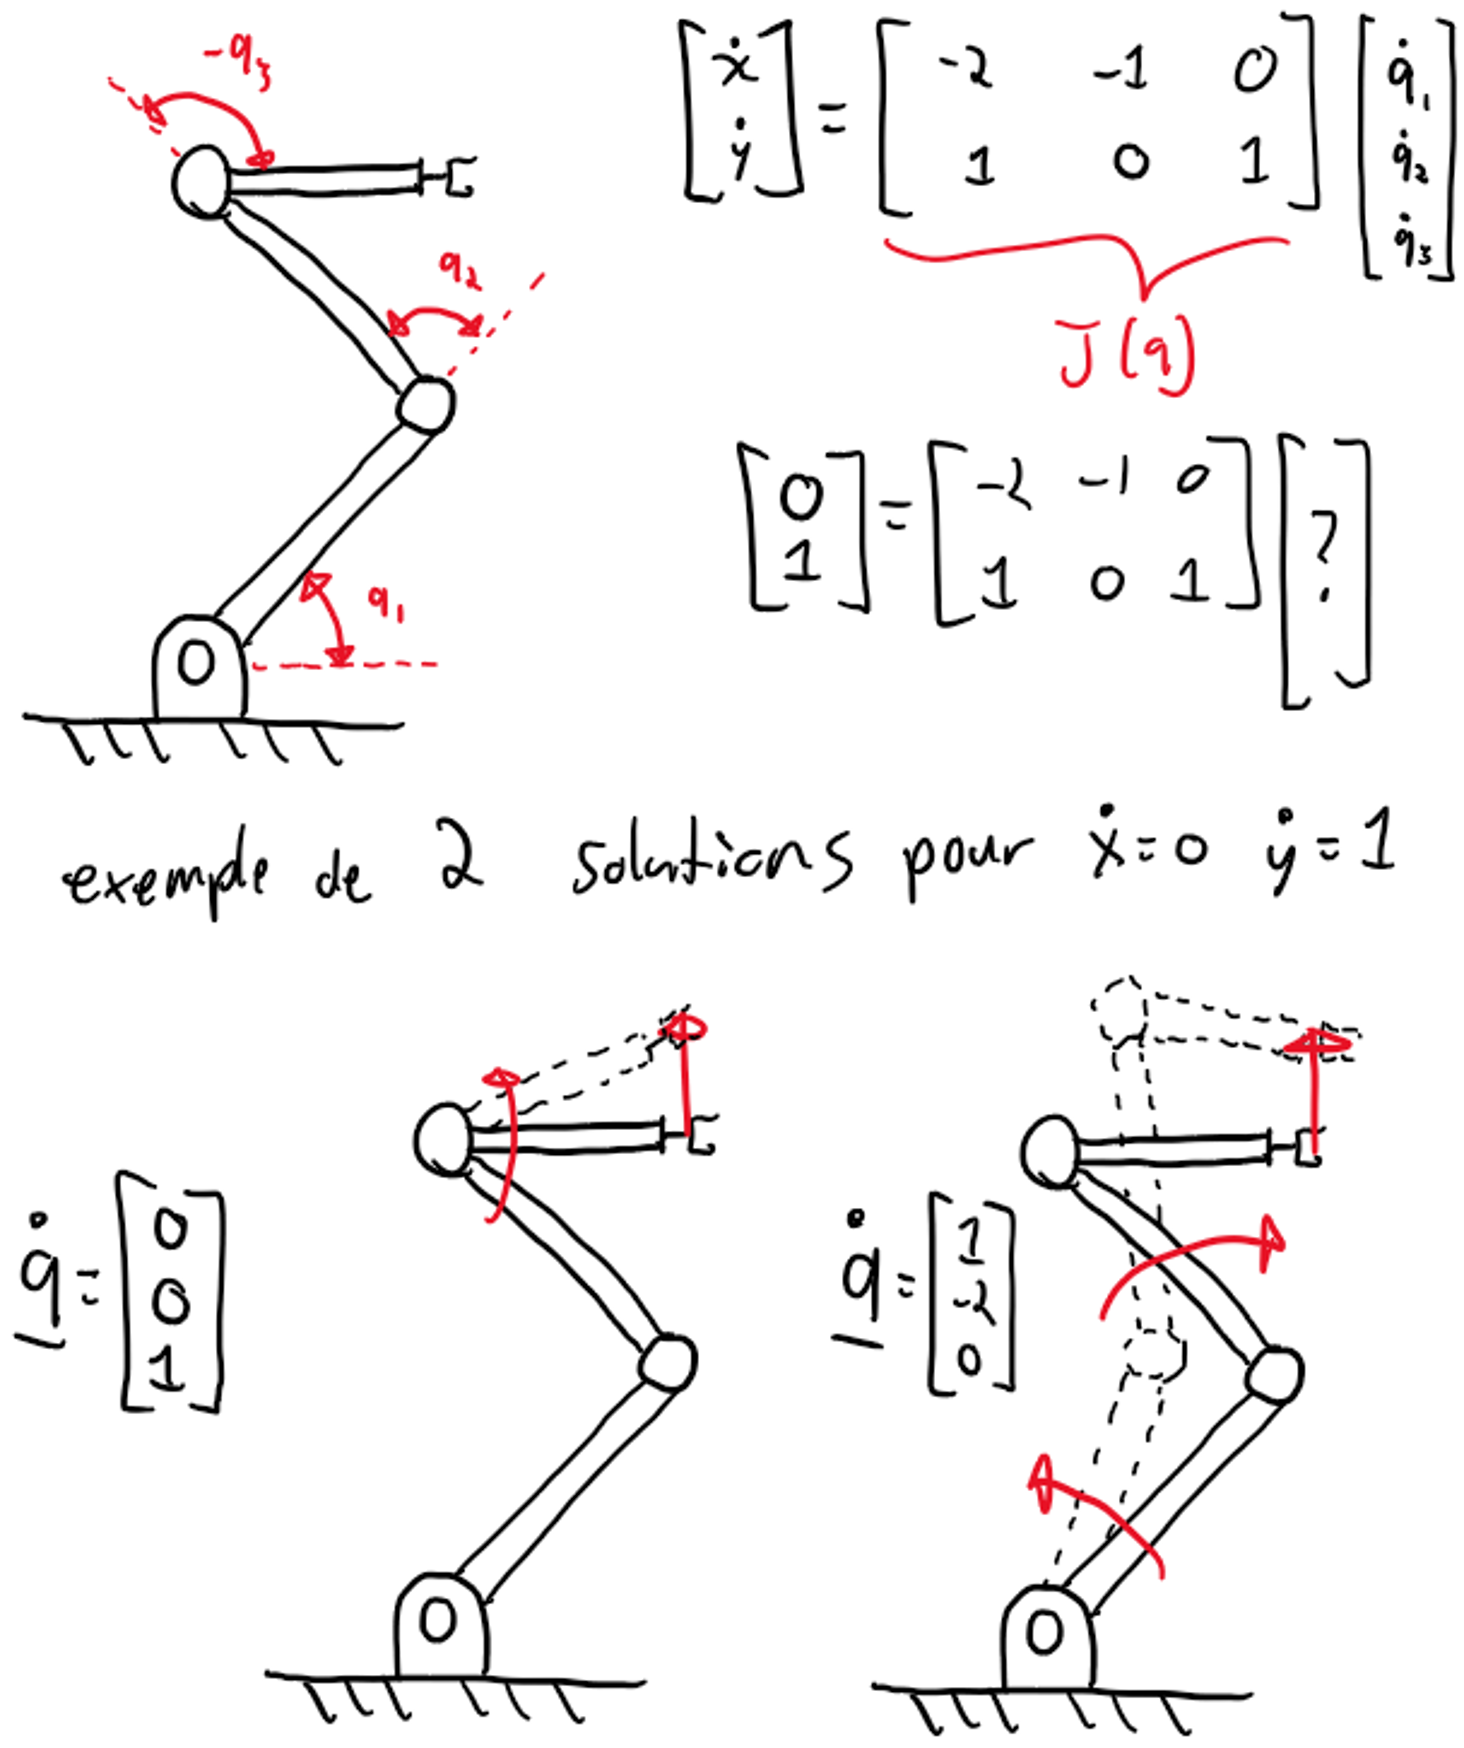
\includegraphics[width=0.65\textwidth]{robot_redo_a.png}
	\caption{Cinématique différentielle inverse d'un robot redondant ($n=3>m=2$)}
	\label{fig:robot_redo_a}
\end{figure}
%%%%%%%%%%%%%%%%%%%%%%%%%%%%%%%%%%
%
%%%%%%%%%%%%%%%%%%%%%%%%%%%%%%%%%%%
%\begin{figure}[H]
	%\centering
		%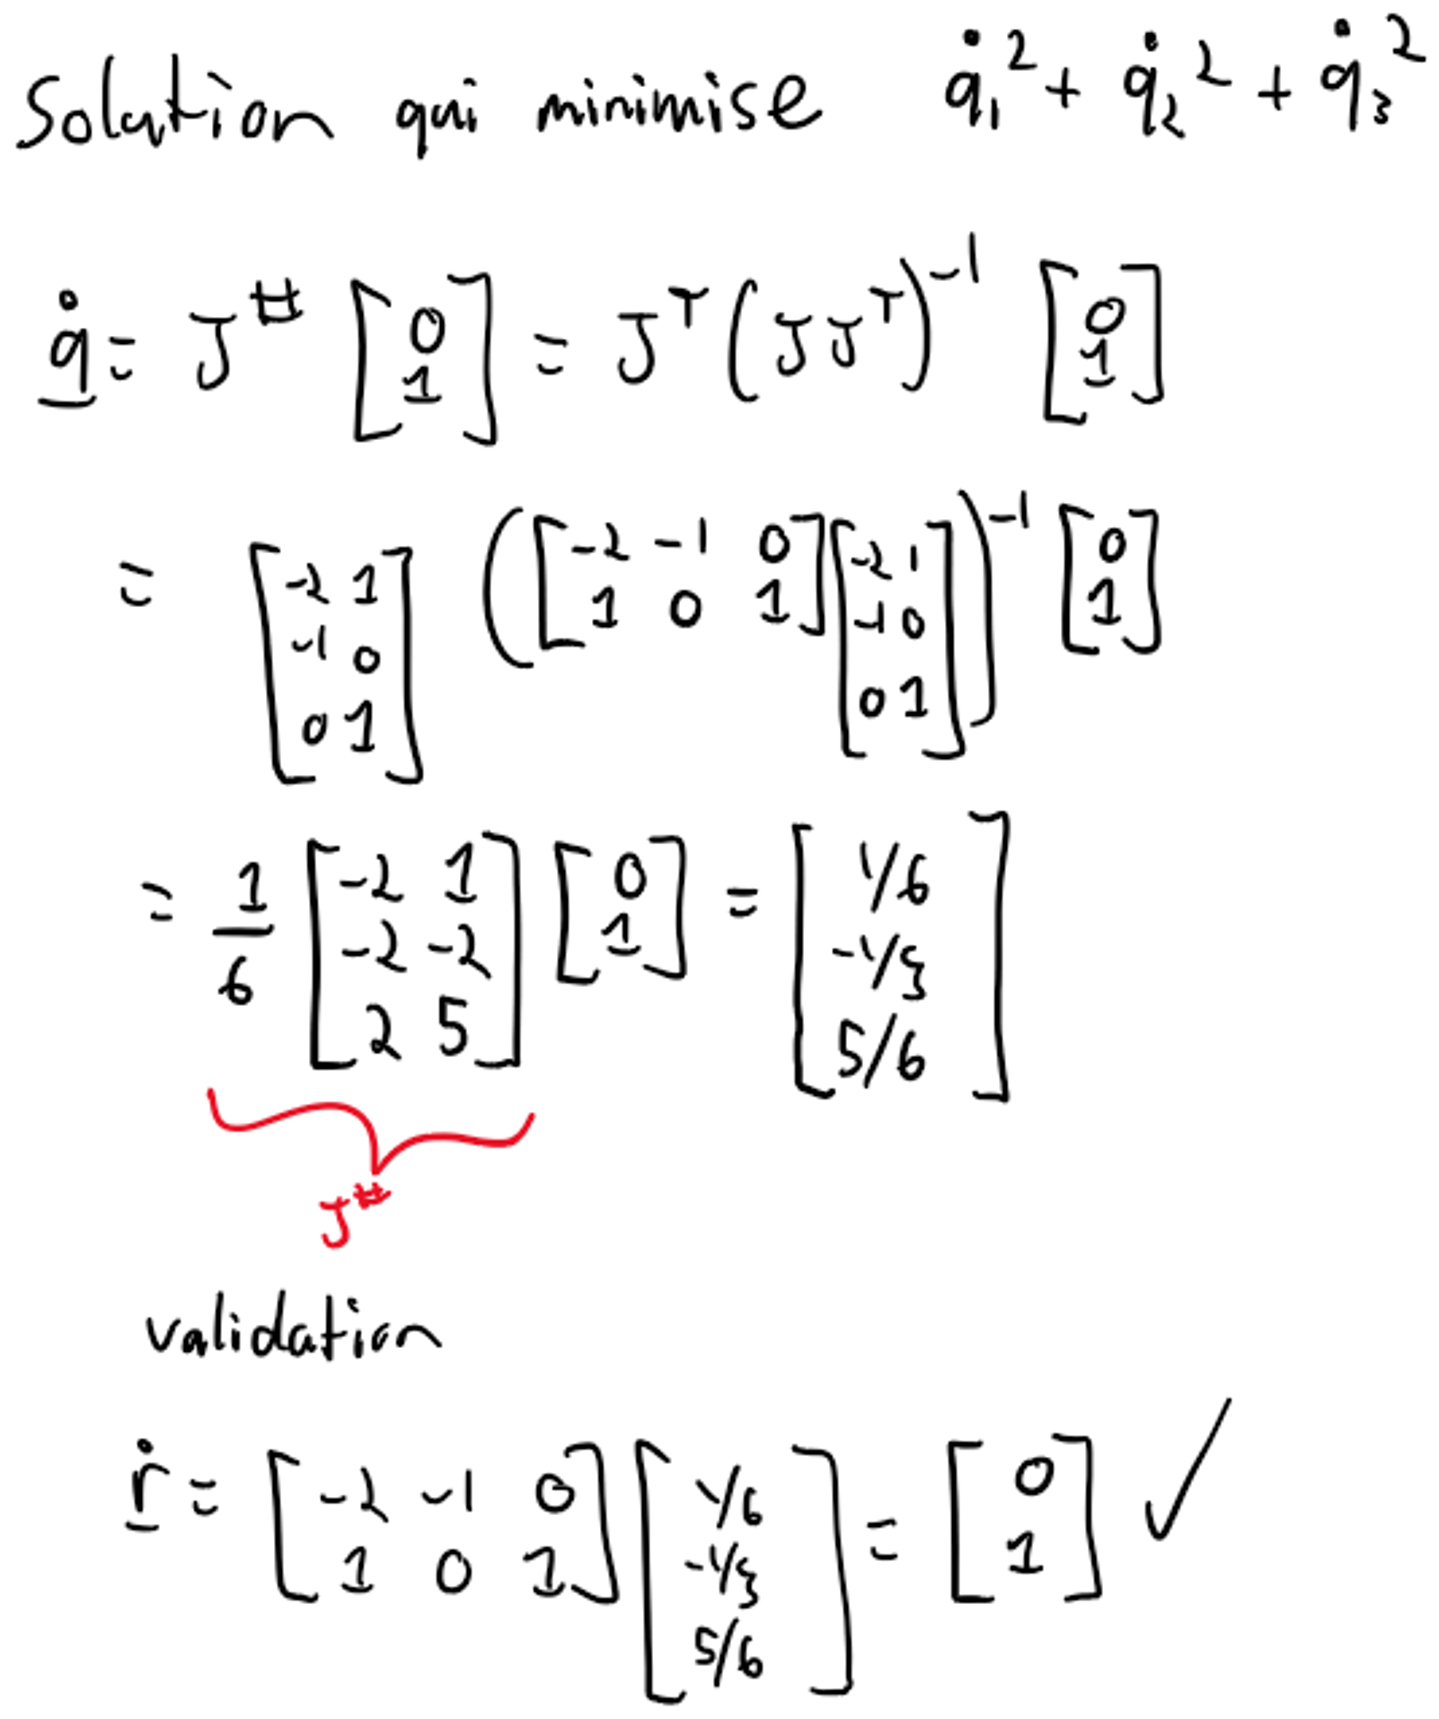
\includegraphics[width=0.55\textwidth]{robot_redo_b.png}
	%%\caption{Co-linéarité des colonnes du Jacobien pour une singularité}
	%\label{fig:robot_redo_b}
%\end{figure}
%%%%%%%%%%%%%%%%%%%%%%%%%%%%%%%%%%%

%%%%%%%%%%%%%%%%%%%%%%%%%%%%%%%%%%
\begin{figure}[H]
	\centering
		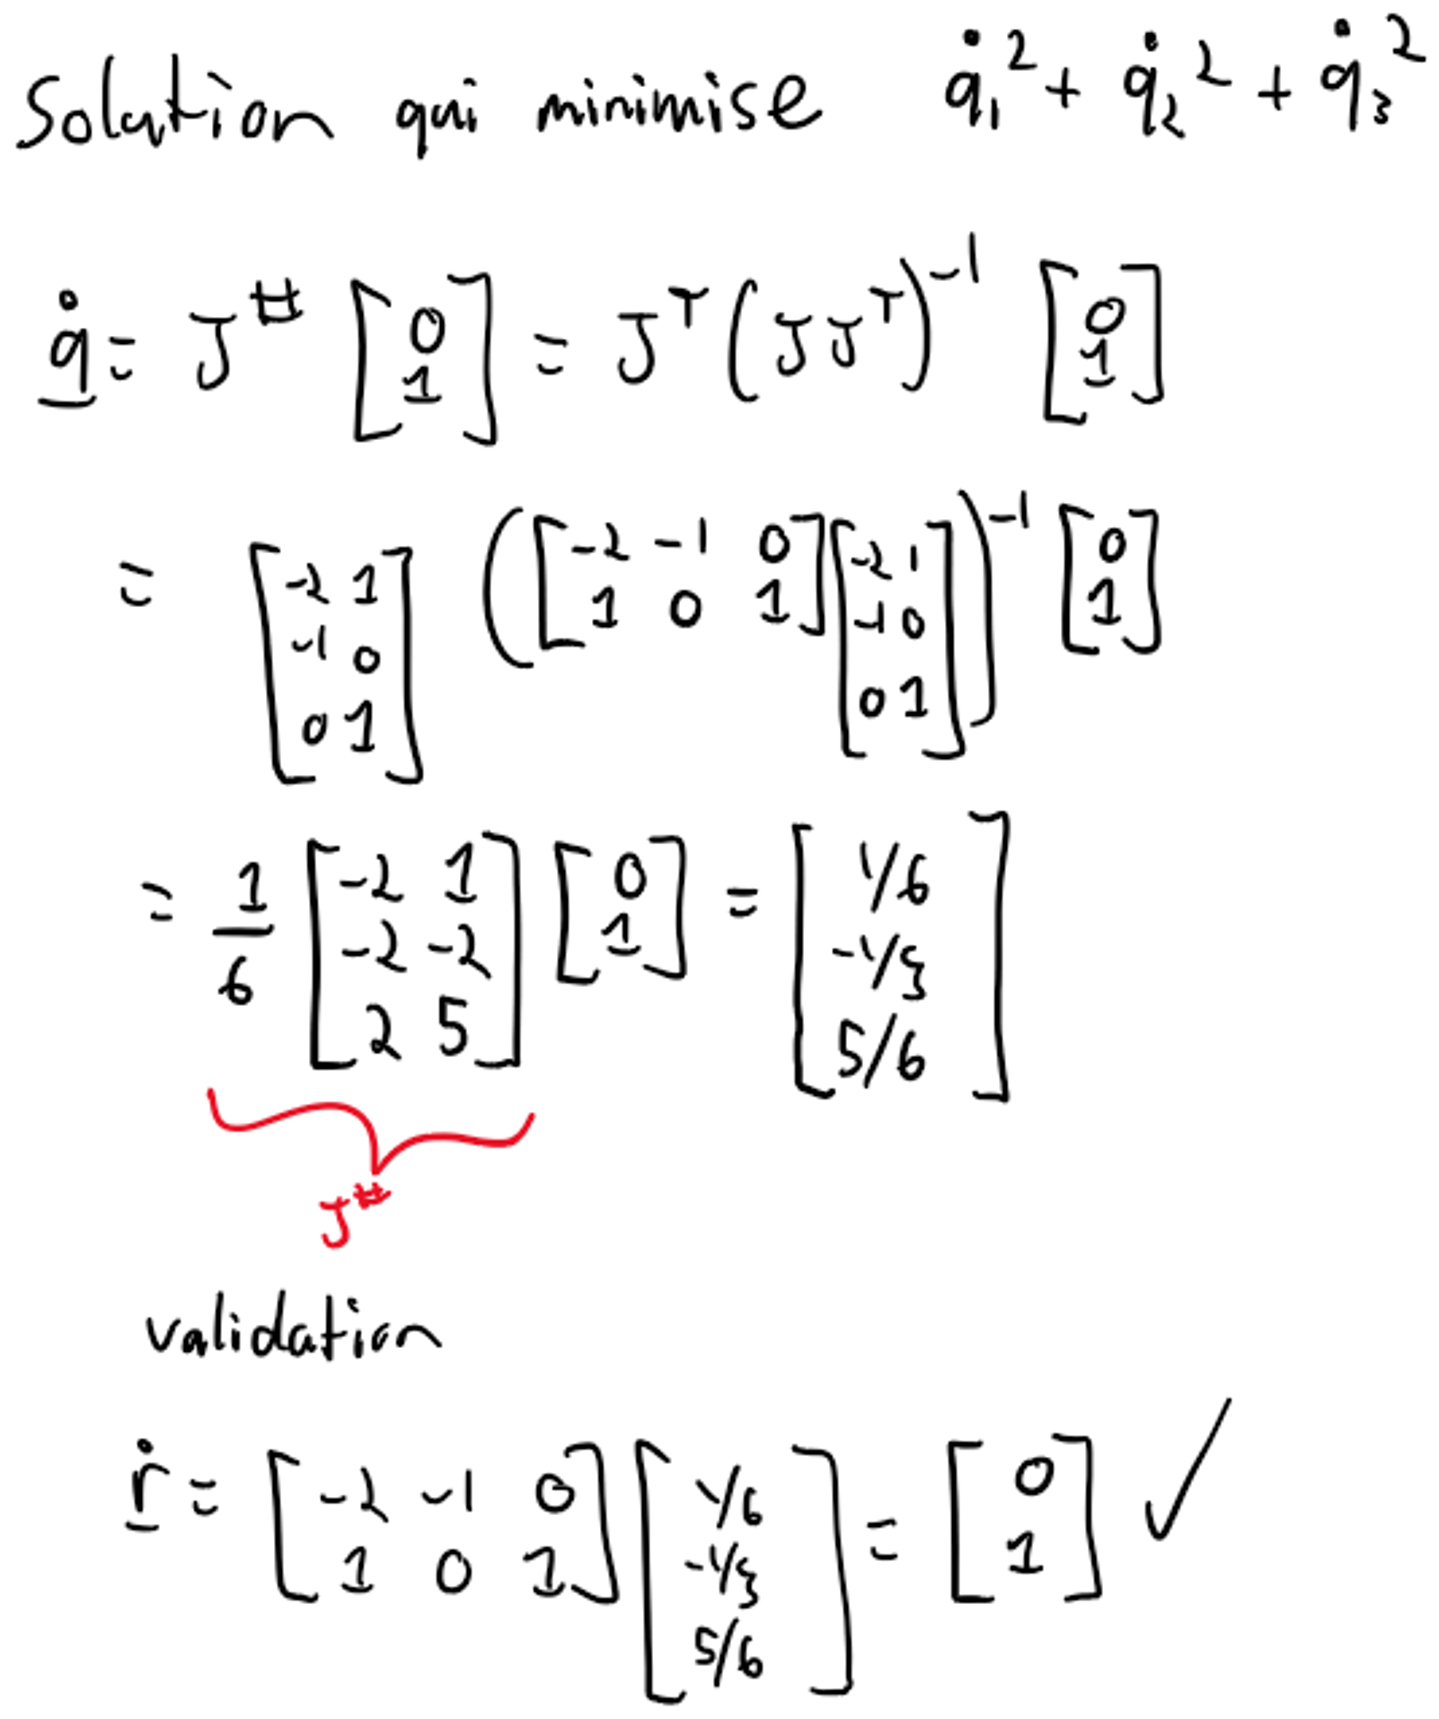
\includegraphics[width=0.55\textwidth]{robot_redo_b.png}
		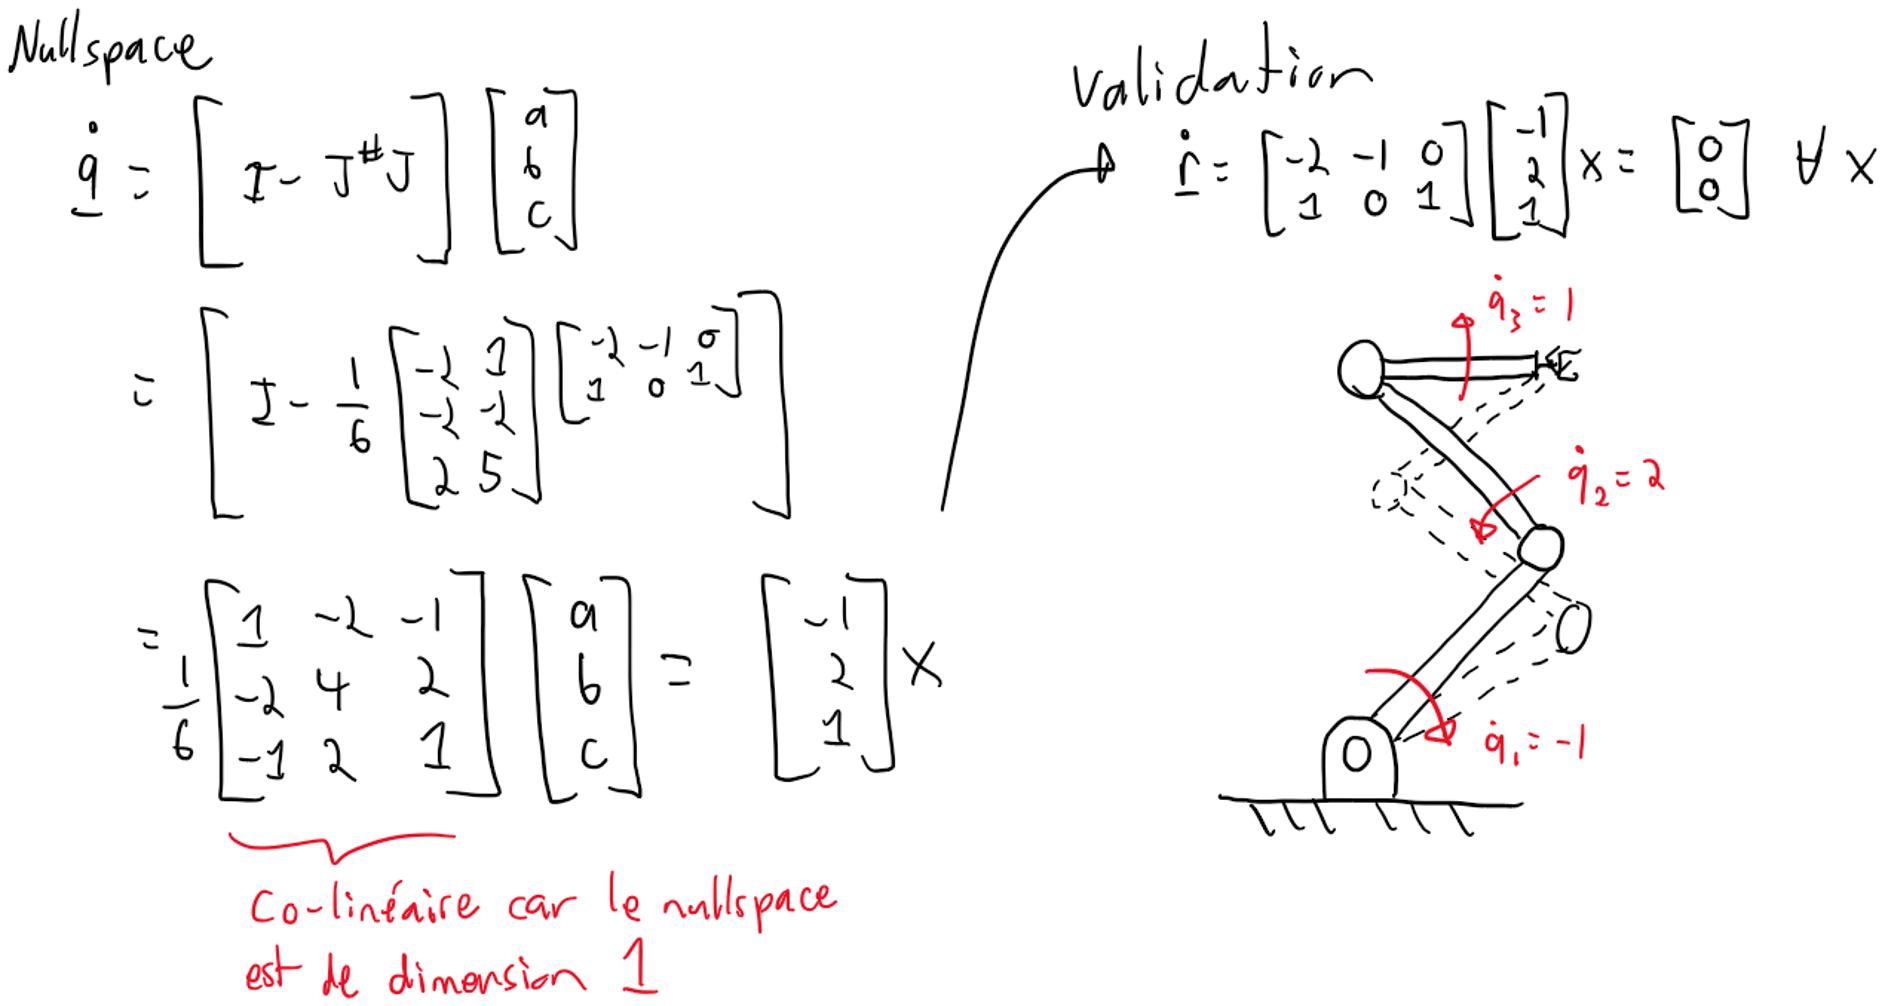
\includegraphics[width=0.95\textwidth]{robot_redo_c.png}
	\caption{Cinématique différentielle inverse d'un robot redondant: solution optimale et nullspace}
	\label{fig:robot_redo_c}
\end{figure}
%%%%%%%%%%%%%%%%%%%%%%%%%%%%%%%%%%




\newpage
%%%%%%%%%%%%%%%%%%%%%%%%%%%%%%%%%%%%%%%%%%%%%%%%%%%%%%%%%%%%%%%%%%%%%%%%%%%%%%%%%%%%%%%%%%%%%%%%%%%%%%%%%
\subsection{Cinématique différentielle inverse pour une situation sur-contrainte}
\label{sec:overconstraintrobot}
%%%%%%%%%%%%%%%%%%%%%%%%%%%%%%%%%%

Si le nombre d'entrées $n$ est plus petit que le nombre de sorties $m$ : 
%%%%%%%%%%%%%%%%%%%%%%%%%%%%%%%%%%%
\begin{align}
n < m
\end{align} 
%%%%%%%%%%%%%%%%%%%%%%%%%%%%%%%%%%%
avec 
%%%%%%%%%%%%%%%%%%%%%%%%%%%%%%%%%%%
\begin{align}
n &= dim(\col{q}) = \quad\text{Nombre de DDL du robot} \\
m &= dim(\col{r}) = \quad\text{Coordonnées de l'espace de la tâche} 
\end{align} 
%%%%%%%%%%%%%%%%%%%%%%%%%%%%%%%%%%%
le problème de cinématique différentiel inverse est sur-contraint: il n'y a pas de solutions exactes possibles sauf pour un sous-ensemble de déplacements de l'effecteur. Le Jacobien d'une telle situation est rectangulaire, il a plus de rangées que de colonnes:
%%%%%%%%%%%%%%%%%%%%%%%%%%%%%%%%%%%
\begin{align}
\left[ \begin{array}{c}  \\ \\ \dot{\col{r}} \\ \\ \\ 
\end{array} \right]_{m \times 1}
&= 
\left[ \begin{array}{c c c} 
&&\\
&&\\
& J(\col{q}) &\\
&&\\
&&
\end{array} \right]_{m \times n}
\left[ \begin{array}{c} 
\\ \dot{\col{q}} \\ \\
\end{array} \right]_{n \times 1}
\label{eq:uoverconstraintdiffkin}
\end{align} 
%%%%%%%%%%%%%%%%%%%%%%%%%%%%%%%%%%%

Un méthode pratique pour la cinématique inverse dans ce contexte est la méthode des moindres-carré, voir la section \ref{sec:moindrecarre} pour les notions d'algèbre linéaire. L'utilisation de cette méthode permet de calculer explicitement un vecteur solution approximé $\col{\hat{\dot{q}}}$ qui minimise la norme de l'erreur entre une vitesse à l'effecteur désiré et celle obtenue avec la solution approximée. La solution moindre-carrée est calculée ainsi:
%%%%%%%%%%%%%%%%%%%%%%%%%%%%%%%%%%%
\begin{align}
\col{\hat{\dot{q}}} = \left( J^T J\right)^{-1} J^T \, \dot{\col{r}}
\label{eq:overconstraintdiffkinleastsquare}
\end{align} 
%%%%%%%%%%%%%%%%%%%%%%%%%%%%%%%%%%%
qui dans ce contexte donne la solution optimale pour le problème : 
%%%%%%%%%%%%%%%%%%%%%%%%%%%%%%%%%%%
\begin{align}
\col{\hat{\dot{q}}} =  \operatornamewithlimits{argmin}\limits_{\col{\dot{q}}} \left\| J \col{\dot{q}} - \col{\dot{r}} \right\|
\label{eq:overconstraintdiffkinleastsquare}
\end{align} 
%%%%%%%%%%%%%%%%%%%%%%%%%%%%%%%%%%%


\newpage
%%%%%%%%%%%%%%%%%%%%%%%%%%%%%%%%%%%%%%%%%%%%%%%%%%%%%%%%%%%%%%%%%%%%%%%%%%%%%%%%%%%%%%%%%%%%%%%%%%%%%%%%%
\subsubsection{Exemple de cinématique différentielle inverse pour une situation sur-contrainte}


%%%%%%%%%%%%%%%%%%%%%%%%%%%%%%%%%%
\begin{figure}[H]
	\centering
		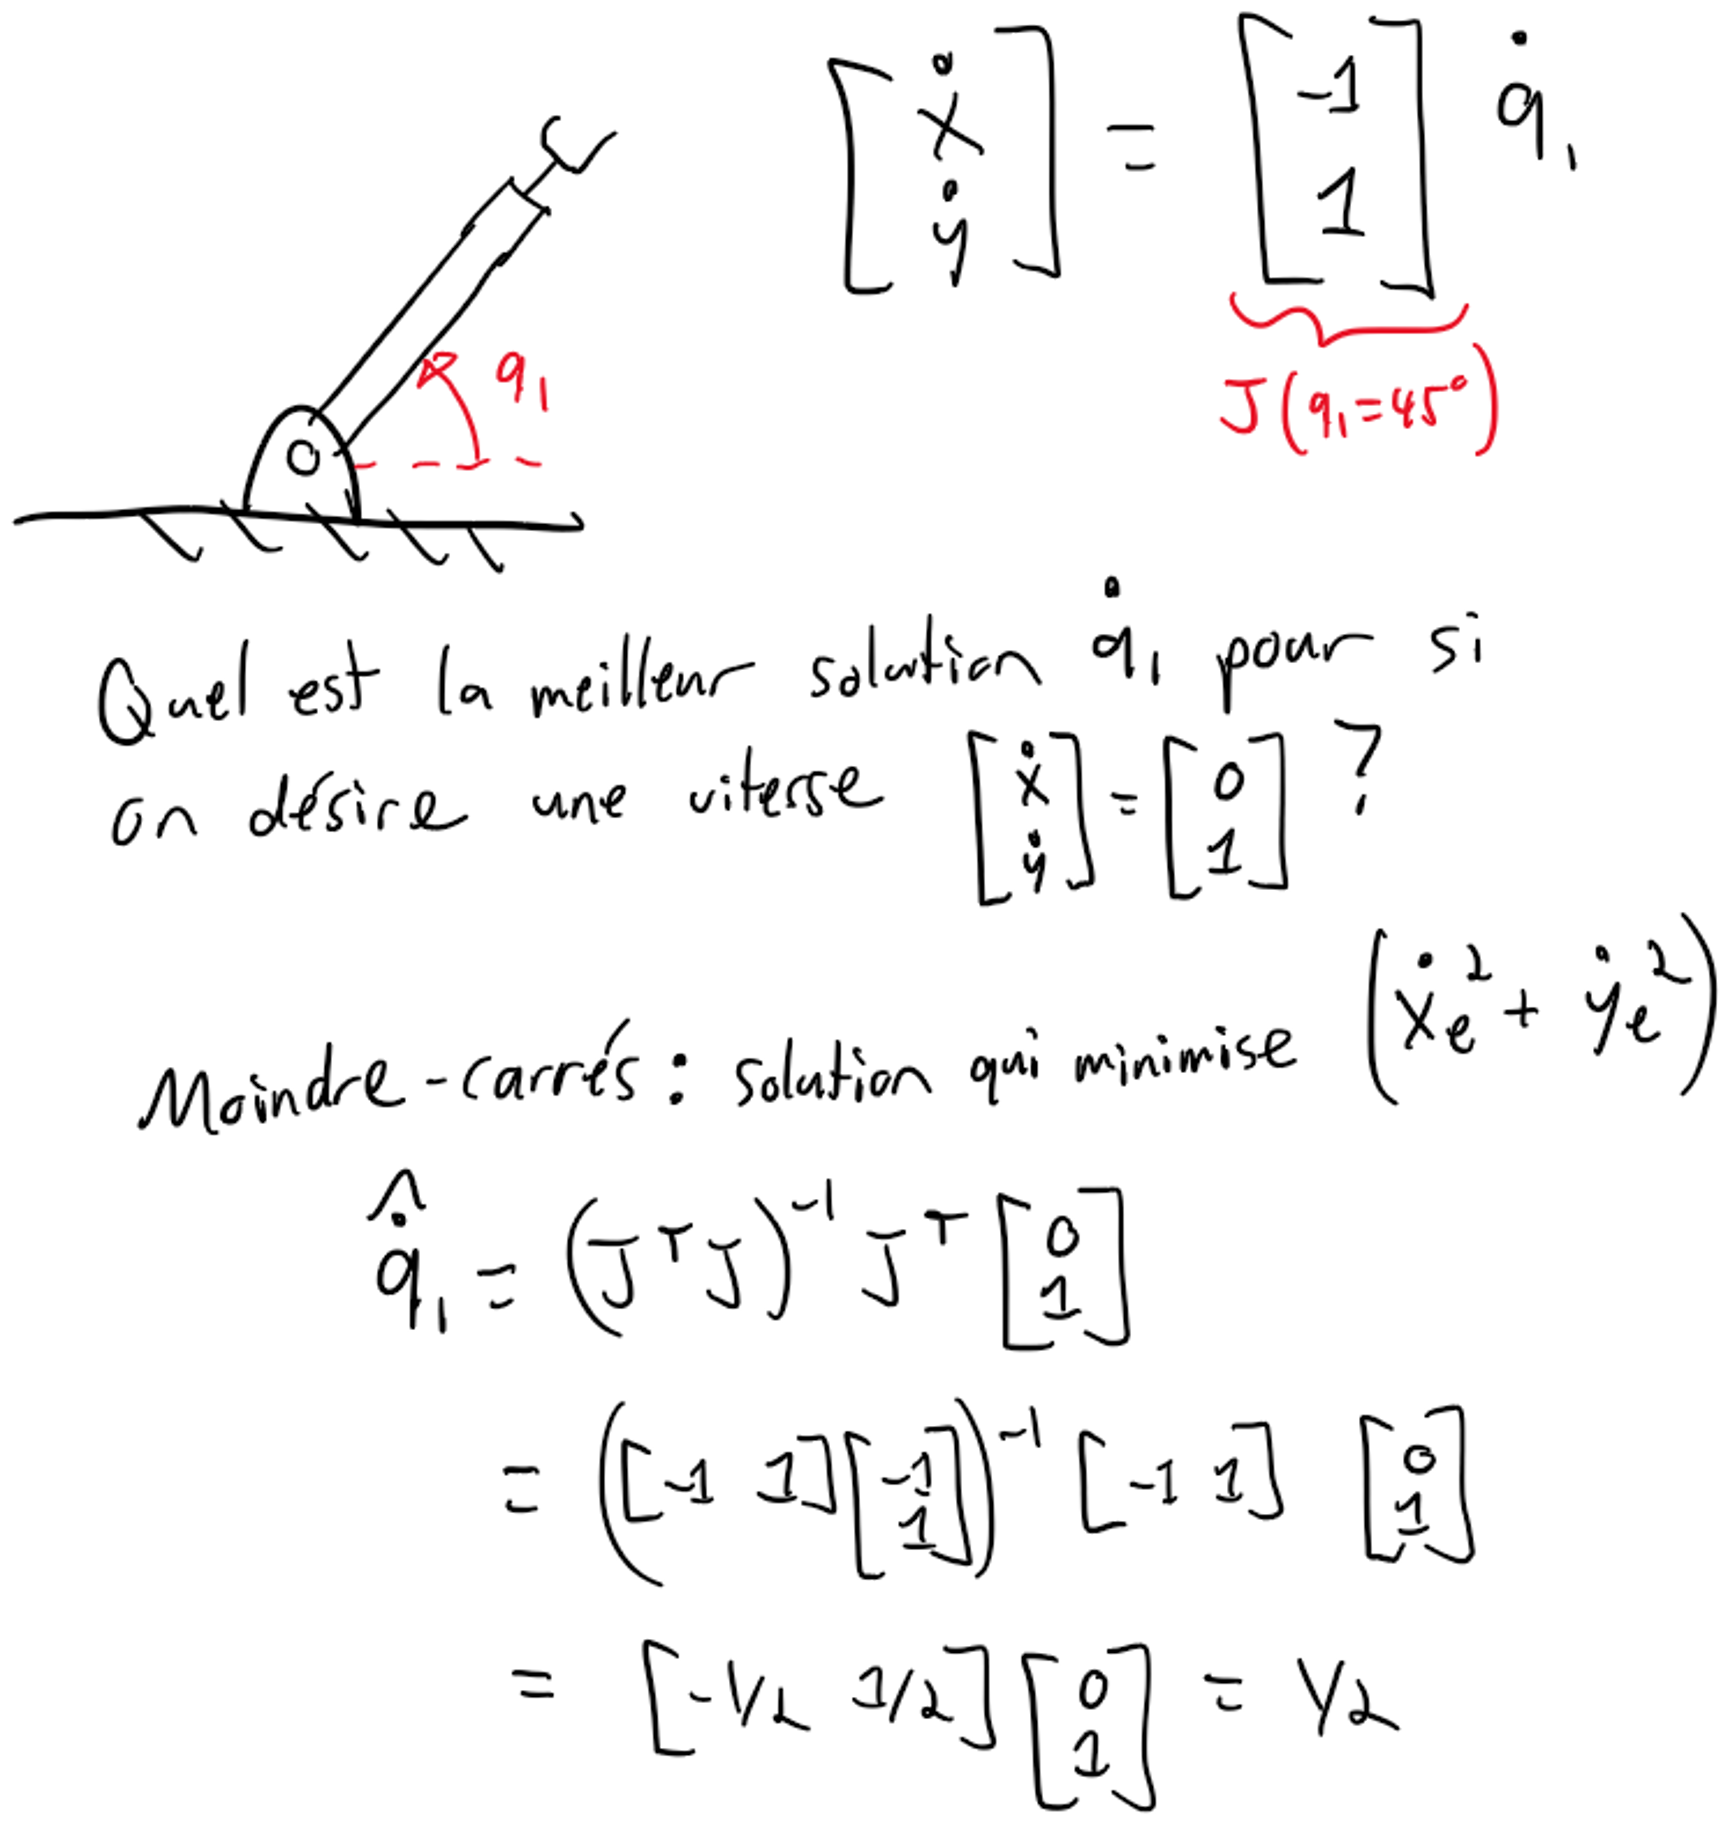
\includegraphics[width=0.55\textwidth]{robot_under.png}
	\caption{Cinématique différentielle inverse pour une situation sur-contrainte ($n=1<m=2$)}
	\label{fig:robot_under}
\end{figure}
%%%%%%%%%%%%%%%%%%%%%%%%%%%%%%%%%%







